\documentclass{sigchi}

% Use this command to override the default ACM copyright statement (e.g. for preprints).
% Consult the conference website for the camera-ready copyright statement.


%% EXAMPLE BEGIN -- HOW TO OVERRIDE THE DEFAULT COPYRIGHT STRIP -- (July 22, 2013 - Paul Baumann)
% \toappear{Permission to make digital or hard copies of all or part of this work for personal or classroom use is 	granted without fee provided that copies are not made or distributed for profit or commercial advantage and that copies bear this notice and the full citation on the first page. Copyrights for components of this work owned by others than ACM must be honored. Abstracting with credit is permitted. To copy otherwise, or republish, to post on servers or to redistribute to lists, requires prior specific permission and/or a fee. Request permissions from permissions@acm.org. \\
% {\emph{CHI'14}}, April 26--May 1, 2014, Toronto, Canada. \\
% Copyright \copyright~2014 ACM ISBN/14/04...\$15.00. \\
% DOI string from ACM form confirmation}
%% EXAMPLE END -- HOW TO OVERRIDE THE DEFAULT COPYRIGHT STRIP -- (July 22, 2013 - Paul Baumann)


% Arabic page numbers for submission.
% Remove this line to eliminate page numbers for the camera ready copy
% \pagenumbering{arabic}


% Load basic packages
\usepackage{balance}  % to better equalize the last page
\usepackage{graphics} % for EPS, load graphicx instead
\usepackage{times}    % comment if you want LaTeX's default font
\usepackage{url}      % llt: nicely formatted URLs

\usepackage{multirow}
\usepackage{ wasysym }
\usepackage{ textcomp }
\usepackage{tabularx}
\usepackage{mathtools}
\usepackage[valuemode=math,unitmode=math]{siunitx}


% llt: Define a global style for URLs, rather that the default one
\makeatletter
\def\url@leostyle{%
  \@ifundefined{selectfont}{\def\UrlFont{\sf}}{\def\UrlFont{\small\bf\ttfamily}}}
\makeatother
\urlstyle{leo}


% To make various LaTeX processors do the right thing with page size.
\def\pprw{8.5in}
\def\pprh{11in}
\special{papersize=\pprw,\pprh}
\setlength{\paperwidth}{\pprw}
\setlength{\paperheight}{\pprh}
\setlength{\pdfpagewidth}{\pprw}
\setlength{\pdfpageheight}{\pprh}

% Make sure hyperref comes last of your loaded packages,
% to give it a fighting chance of not being over-written,
% since its job is to redefine many LaTeX commands.
\usepackage[pdftex]{hyperref}
\hypersetup{
pdftitle={Aesthetic Electronics: Designing, Sketching, and Fabricating through Digital Exploration},
% pdftitle={Ellustrate: Designing, Sketching, and Fabricating Aesthetic Electronics through Digital Exploration},
pdfauthor={LaTeX},
pdfkeywords={SIGCHI, proceedings, archival format},
bookmarksnumbered,
pdfstartview={FitH},
colorlinks,
citecolor=black,
filecolor=black,
linkcolor=black,
urlcolor=black,
breaklinks=true,
}

% create a shortcut to typeset table headings
\newcommand\tabhead[1]{\small\textbf{#1}}

% set up tight list spacing
\usepackage{enumitem} 
\setlist{nolistsep,nosep}

% for toggles
\usepackage{etoolbox}


% CHANGE FROM TOGGLE TRUE TO TOGGLE FALSE TO HIDE COMMENTS
\newtoggle{comments}
\toggletrue{comments}
% \togglefalse{comments}

% Comment region command (from Wesley Willett)
\usepackage[usenames]{color}
\usepackage[usenames,dvipsnames]{xcolor}
\iftoggle{comments} {
  %if we want to show comments
  \newcommand {\jlo}[1]{{\color{magenta}\bf{JLO: #1}\normalfont}}
  \newcommand {\cesar}[1]{{\color{NavyBlue}\bf{CAT: #1}\normalfont}}
  \newcommand {\ep}[1]{{\color{violet}\bf{EP: #1}\normalfont}}
  \newcommand {\mira}[1]{{\color{Orange}\bf{MD: #1}\normalfont}}
  \newcommand {\wil}[1]{{\color{Blue}\bf{WL: #1}\normalfont}}
  \newcommand {\danny}[1]{{\color{Red}\bf{DK: #1}\normalfont}}
}{
  %if we don't want to show comments
  \newcommand {\jlo}[1]{}
  \newcommand {\cesar}[1]{}
  \newcommand {\ep}[1]{}
  \newcommand {\mira}[1]{}
  \newcommand {\wil}[1]{}
  \newcommand {\danny}[1]{}
}

\newenvironment{myquote}{\list{}{\leftmargin=0.01\textwidth \rightmargin=0.01\textwidth}\item[]}{\endlist}
\newcommand*{\quoted}[1]{{\small{\fontfamily{cmss}\selectfont{#1}}}}
\newcommand*{\layer}[1]{{\textbf{\small{\fontfamily{cmss}\selectfont{#1}}}}}
\newcommand*{\participant}[1]{{\textbf{\small{\fontfamily{cmss}\selectfont{#1}}}}}
\newcommand*{\factor}[1]{{\textbf{\small{\fontfamily{cmss}\selectfont{#1}}}}}
\newcommand*{\nt}[1]{{\textbf{\small{\fontfamily{cmss}\selectfont{#1}}}}}
\newcommand*{\code}[1]{{\small{\fontfamily{cmss}\selectfont{#1}}}}




% End of preamble. Here it comes the document.
\begin{document}

\title{Aesthetic Electronics: Designing, Sketching, and Fabricating through Digital Exploration}
% \title{Ellustrate: Designing, Sketching, and Fabricating Aesthetic Electronics through Digital Exploration}

% \title{Ellustrate: Enabling Aesthetic Design and Fabrication for Silver, Copper, and Conductive Thread Circuits}
% \title{Ellustrate: Enabling Visual Circuit Design and Fabrication for Multiple Materials}

% \numberofauthors{1}
% \author{
%   \alignauthor Anonymized for Submission\\
%     \affaddr{...}\\
%     \affaddr{...}\\
%     \email{...}
% }
\teaser{
  \vspace{-20pt}
  \centering
  \includegraphics[width=\linewidth]{figures/teaser.pdf}
  \caption{
    a) A painting made with conductive silver ink, b) a copper tape object, c) a conductive thread embroidered pattern. }
    \vspace{-8pt}
  \label{fig:teaser}
}

\maketitle

\begin{abstract}
As interactive electronics become more intimate and personal, the design of the circuitry has developed a more playful and creative aesthetics as well. Circuit sketching and design multidimensional activity combining the arts, crafts, and engineering, broadening participation of electronic creation to include designers of diverse backgrounds. In order to support this design ecology, we present Ellustrate, a digital design tool that enables the functional and aesthetic design of electronic circuits with multiple conductive and dielectric materials. Additionally, Ellustrate guides users through all essential fabrication and debugging steps towards realizing their aesthetic electronic design. In a formal user study, we demonstrate how Ellustrate facilitates a new electronic design conversation that combine electronics, materials, and visual aesthetic considerations. 

% Circuit sketching has gained traction in creative communities as a method of democratizing circuit creation, diversifying the materials and techniques used to make unique, critical artifacts. In order to support this design ecology, we present Ellustrate, a digital design tool that enables the functional and aesthetic design and fabrication of electronic circuits.
% Ellustrate incorporates a holistic design cycle in a digital design tool which guides users through all essential steps towards realizing their electronic ideas. The tool provides designers with a digital assistive artboard which aids users with constructing electrically-valid circuits through a set of visual rules. Using a connectivity graph, we can provide step-by-step material-specific fabrication and debugging instructions for each design.
% In a formal user study, we show how Ellustrate enables a new circuit aesthetic that operates beyond efficiency, and can serve as a scaffold for designers and artists to incorporate electronic design in their everyday practice.
% We discuss how such tools that enable material-first exploration can support growing online communities. 


% and incorporates story-telling and new mental model.

% democratize electronic design to include designers and artists and examine the aesthetic value of circuit design beyond
% Ellustrate provides multi-material support and design-focused drawing tools tailored for aesthetically-driven functional circuit design. 
% Within the Ellustrate design tool, designers receive immediately feedback and corrections on their circuit design as they create their electronic artwork.
% Beyond the electrical and visual design, Ellustrate also offers step-by-step guidance on fabricating and debugging.

\end{abstract}
\keywords{
	design tool; sketching circuits; fabrication  \newline
}

\category{H.5.m.}{Information Interfaces and Presentation (e.g. HCI)}{Miscellaneous}

\section{Introduction}
The landscape of electronics is rapidly changing - devices are becoming smaller and thinner exponentially, often taking on unexpected form factors. Electronic circuits are now being printed directly on the device housing to conserve internal space, and electronics on ultra-thin wearables devices are directly visible to the user. 
The sentiment of the blending of functional and structural materials are echoed by the Radical Atoms vision, which calls for “new material design principles” that “treat objects as homogeneous entities with the ability to change their properties” (cite radiacal atoms).  In this paper, we use the term \textit{Aesthetic Electronics} to describe a class of electronics that enhance and facilitate interactive experience by taking aesthetics and electronic functions as intercorrelated design variables. A set of capacitors with shapes of interdigitated ocean waves could be used as a capacitive slider, and electrical traces that appears to be tree branches could be appreciated as an augmented painting. Modifying shapes, lengths, and material used are going to affect traditional electrical design variables such as resistance, capacitance, and inductance. Having the fluency over the affordance of materials is paramount in creating the aesthetic electronic design that addresses all the function and aesthetic requirement in a well-balanced way. 

In Ellustrate, we focus on the creation of a subgroup of aesthetic electronics - aesthetic circuits. We believe electrical traces to be the design element that is currently the most restricted by traditional aesthetic guideline. Aesthetic circuits can be prototyped with a process named Sketching Circuit, a design and fabrication process that enables the creation of physical circuit with craft materials first proposed by Qie el al. It is popular among makers and designers with skills in sketching and crafting but little experience with electronics, and we believe it to be the best first step to broaden the definition of electronic design~\cite{qi_sketching_2014, qi_stickers_2015}. The greatest strength of sketching lies in its natural and intuitive process shared by professional electrical engineers and artists alike - this shared charcteristic can greatly empower early learners to create function circuits. The sketching circuits process has shown to be increase participation of electronic design from diverse population, remove negative stigma associated with circuits, and motivate early learners. Moreover, the ability to incorporate these circuits into their own craft generates unexplored design opportunities and possibilities. 
Drawing and sketching play a critical role within the development of user interfaces. Sketching has shown to bring interesting elements to hardware prototyping, sparking creative innovations within the Maker community. 
Although sketching circuit has many benefits in initial design and early electronic education, it is not explored by supported by many electrical digital design tools.


Various research fields have taken notice of the circuit sketching trend as well, creating various conductive materials (i.e silver, graphite, copper) that can be applied on paper in ways similar to a regular pen~\cite{russo2011pen}. Advances in materials have enabled a new class of circuits that are ``sketchable''. While ease of use of the conductive pen, copper tape, and conductive threads, has enabled many creative crafting projects, we believe the complexity and creativity in electronic craft can be further augmented by providing two critical elements - a digital sandbox and assistance for physical creation. 

%The traditional circuit design aesthetic is mostly influenced by efficiency - how to pack as many lines as possible in shortest distance from one component to another. This is an artifact of the huge demand on miniaturization of electronics and the exponentially increasing burden on electronics to conserve valuable board space. The industry-standardized interest in optimizing for speed and space have influenced early circuit education, even when optimized performance is not as big of a concern compared to eliciting interest and retaining learners.
In most circuit design tool, the final layout of the circuitry create the straight-line, efficiency-focused, design.
Even in design tools that focus on entry-level circuit making, such as 123D Circuits and Fritzing, the functions for drawing the final printed circuit board layout still favor the traditional straight-line aesthetics.
While this tried-and-true layout method is extremely valuable, it also limits how electronics and circuits are viewed - something pedantic instead of creative. Despite the tremendous benefits brought to electronic creation and learning circuit sketching, the process has remained restricted to a physical classroom setting. Ellustrate aims to democratize the electronic design process to include artists and designers with no prior circuit knowledge. 
Ellustrate differs from most circuit design tools in a number of ways: a) it balances concerns of electronic validity and expressive design, b) it integrates the human back into the fabrication process, shown in prior work to improve engagement with techniques and process, and c) provides debugging assistance to aid users with correcting improperly fabricated circuits. \jlo{add tie to Figure 2, expand contribution - to include fomrative study and formal user study}\cesar{+ user study}

% \jlo{Sketching is an integral part of design - in both visual design, and software and hardware engineering design. Digital design tools that aid in physical design have been studied extensively, and their benefits to the final physical design have been well documented. (notes to be flushed out: Material exploration - the ability to think of atoms and bits as clay - traces are not just automatic connections but of varying resistance and other properties - device physics thinking...)}
% As electronic devices become more intertwined and intimate with users, the internal making of them becomes more naked and transparent. Along with the advent of structural electronics, where circuit traces and components are printed on housing of an electronic device, and wearable electronics, where electronics and active components are part of the fashion aesthetics, the ability to inject visual design into functional electronics become increasing important.

\begin{figure}[t]
\centering
  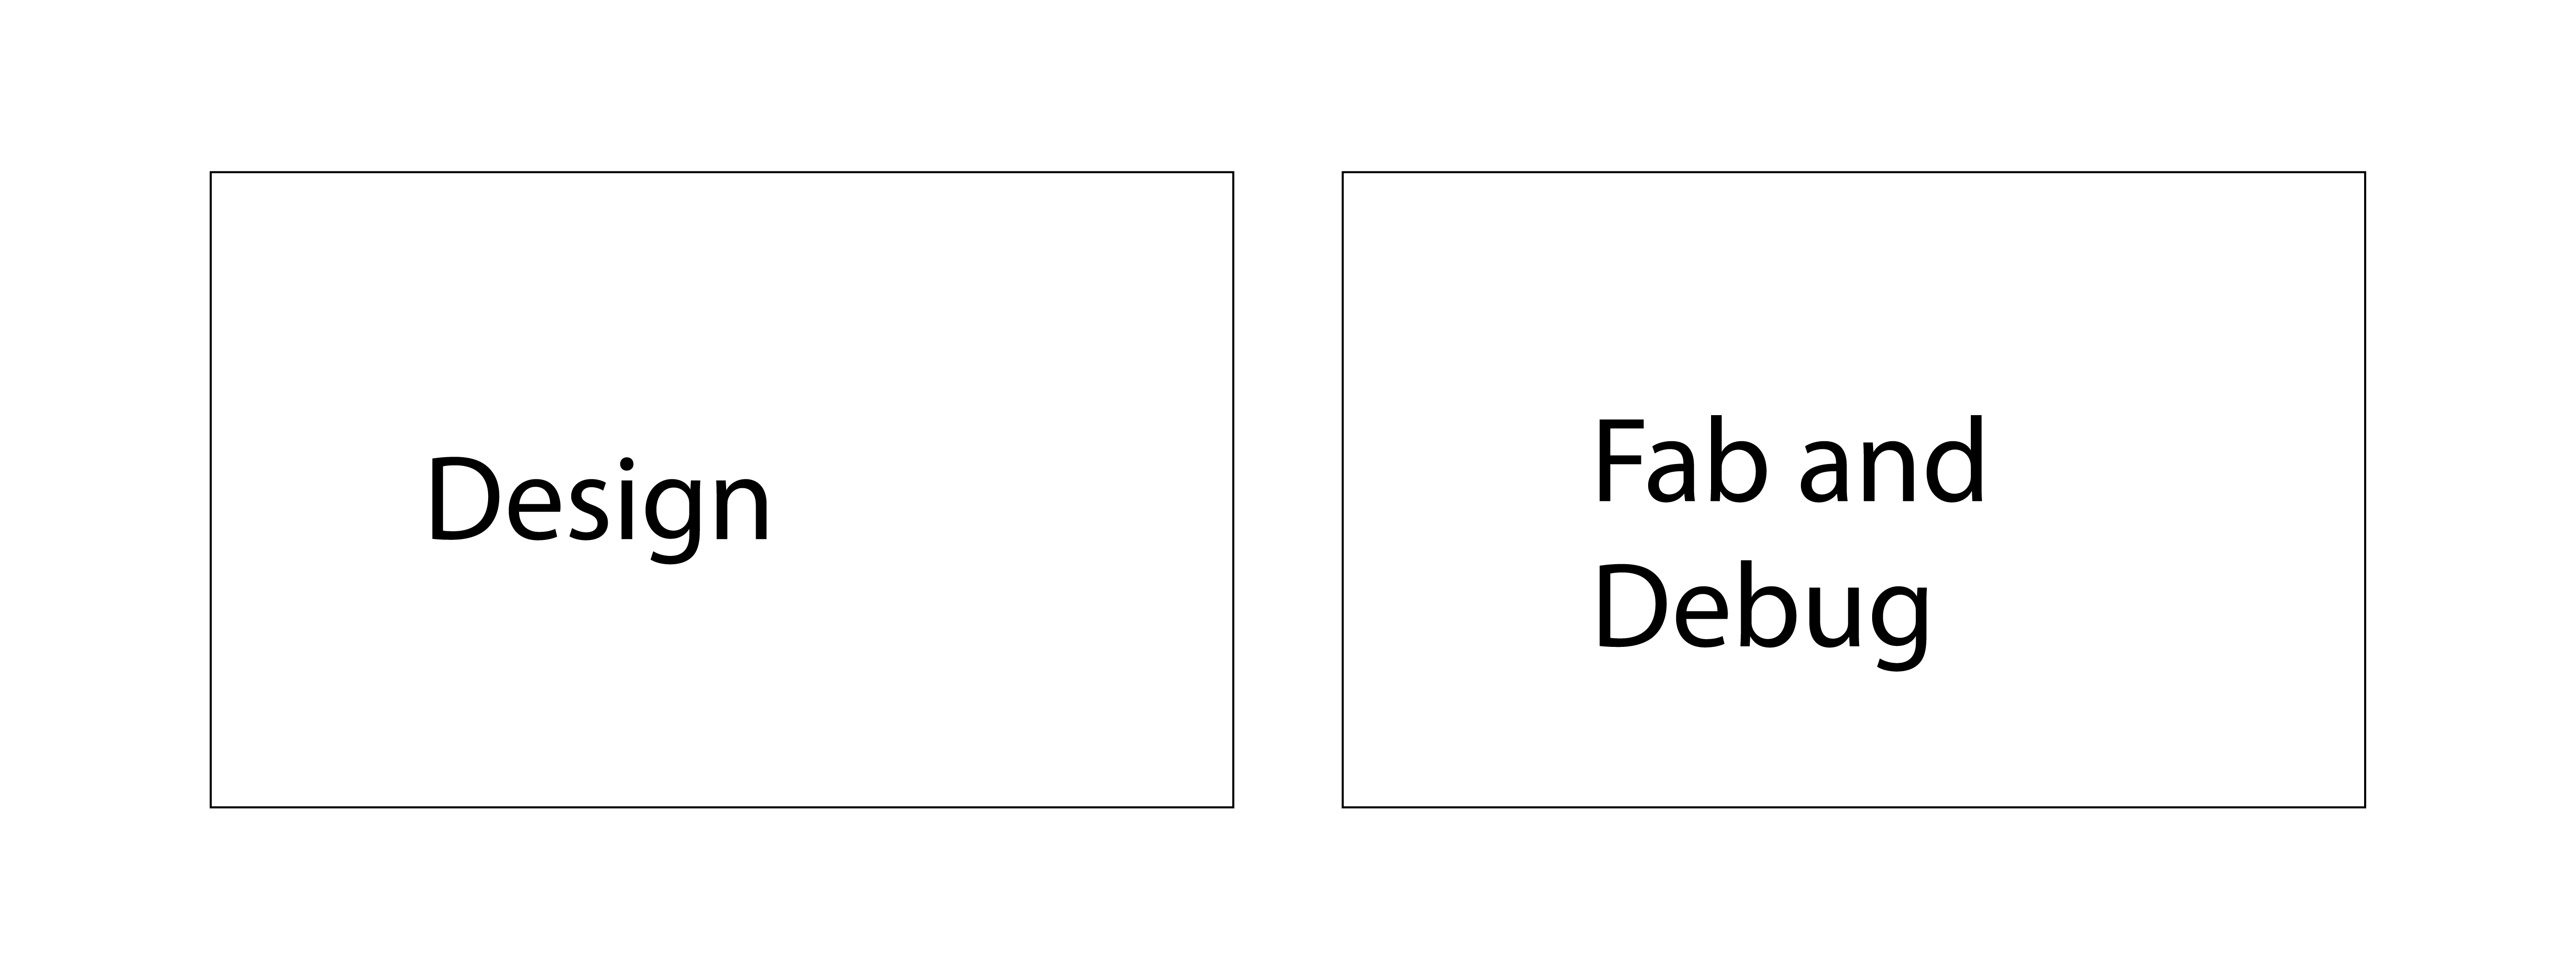
\includegraphics[width=\linewidth]{figures/Ellustrate_figures_process_flow.jpg}
  \caption{A comparison of design tool features. Ellustrate provides coverage for both digital design and circuit design concerns. }~\label{fig:process_flow}
  \vspace{-16pt}
\end{figure}


\section{Related Work}
To create a digital tool that enables the physical creation of physical circuits, we based our work on established research on nontraditional circuits and electronics, as well as relevant digital tools. 

\begin{figure}[t]
\centering
  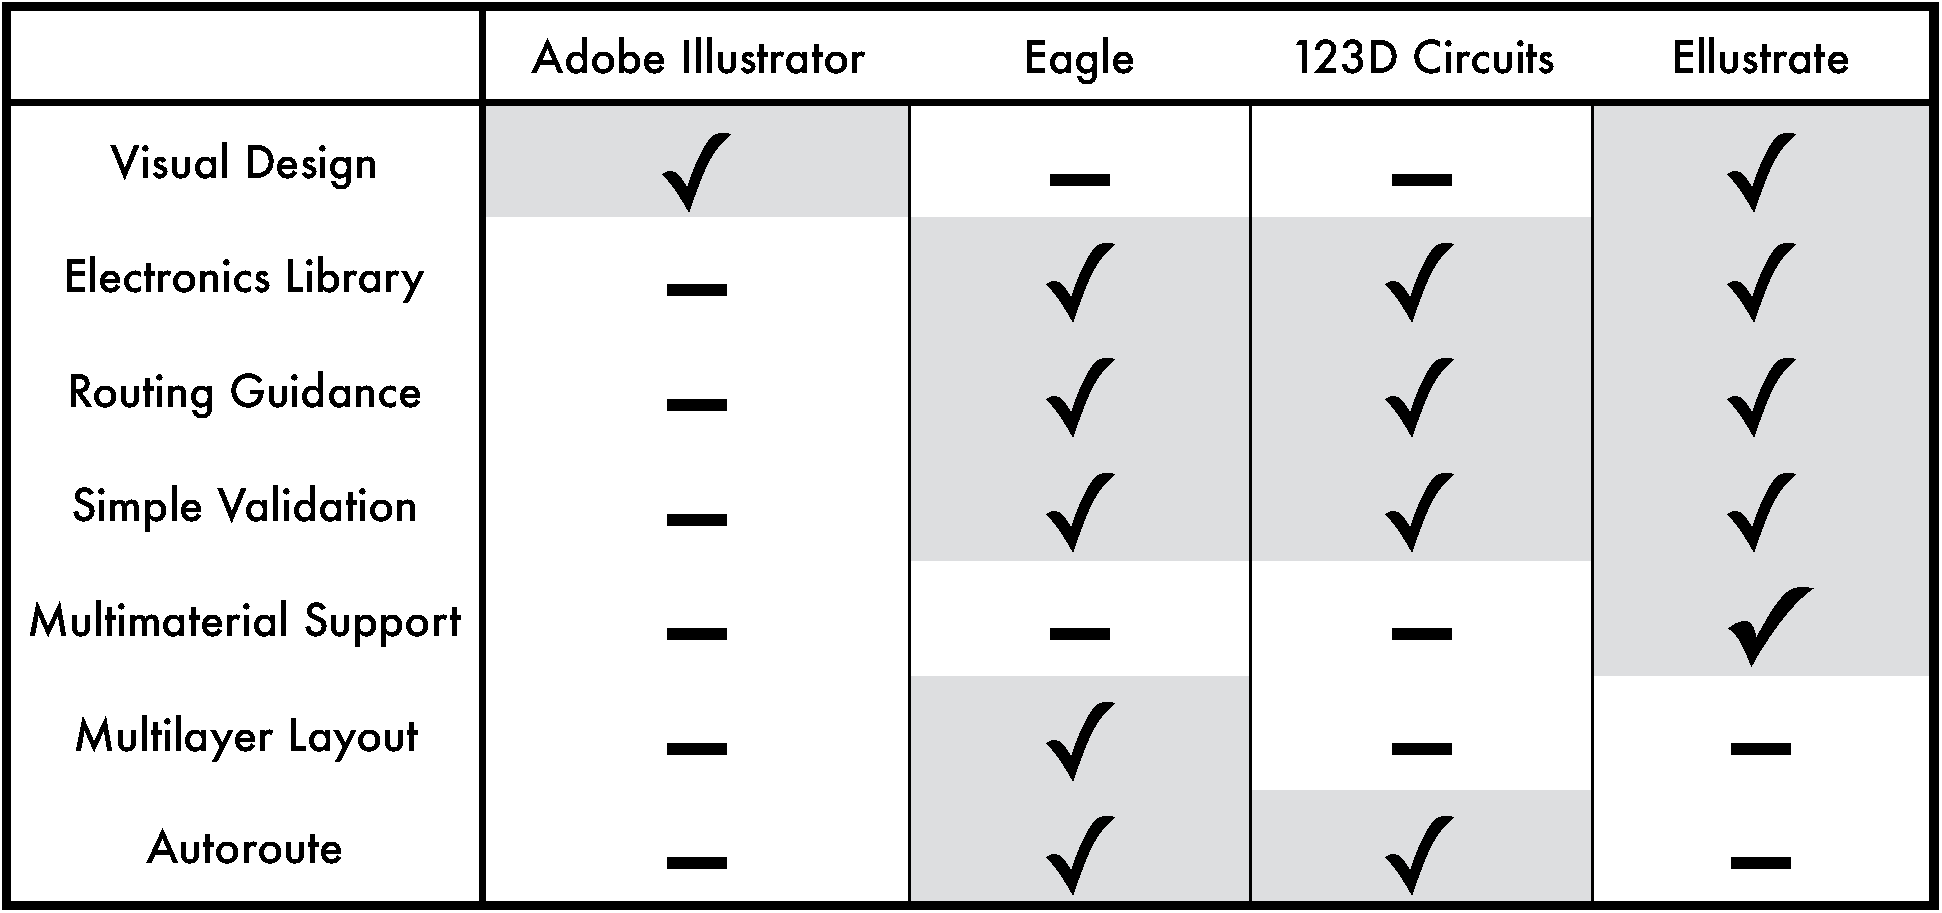
\includegraphics[width=1\columnwidth]{figures/comparative_table.pdf}
  \caption{A comparison of design tool features. Ellustrate provides coverage for both digital design and circuit design concerns. }~\label{fig:comparison_table}
  \vspace{-16pt}
\end{figure}

\subsection{Sketching Electronics on Familiar Materials}
By fabricating electronics on paper, a material that most people are familiar with, users can explore electronic design using a familiar skill set.  Augmenting such common everyday materials with power, lights, and motions has been shown to introduce a sense of wonder that resonates with people of diverse ages and backgrounds~\cite{karagozler_paper_2013}(cite Jie Qi popup book, SMA augment). Furthermore, the role of these materials in everyday life has been shown to be a natural platform for story-telling with electronics. As such, incorporating familiar materials in circuits has altered the design landscape leading to more natural, organic, and novel circuit layouts.
As more conductive and non-conductive materials develop, as does the complexity of understanding the unique electronic intricacies of each material.  Ellustrate aims to support the circuit sketching practice by providing a digital design tool that provides support for working with different materials and encourages an aesthetic exploration of circuit designs.

% Qi et al. cited the expressive medium as the main reason for the successful recruitment of a diverse population who participated in the sketching circuit workshop.
% Buechley et al. and Qi et al. expanded upon the story-telling narrative of paper circuits by leveraging sketching on paper at the onset of the creative ideation. 
% By utilizing the familiarity of a regular pencil, sketching circuits was able to combine the ideation process for both circuit and art design under one platform. (reword).  \cesar{this is too over-reaching}
 % and complement the visual design of the work.



\subsubsection{Digital Sketching Tools} 
Since sketching is such an important element of early stage design, many digital tools have been created to facilitate this process. These tools transform sketches into some form of prototype for the final design by decomposing and recognizing domain-specific symbols and lines. In SILK and SATIN, Landay et al. and Hong et al. investigate a set of software support functions for sketching user interfaces, website design, and simple logic circuits. The two tools generate a final design by ``cleaning up'' imperfections in the hand-drawn sketches - short, overlapping lines are combined, strokes are straightened, and imperfect symbols of logic gates are corrected. The traces between the elements are oftent reduced to the the shortest straight path possible. (talk about Kirchhoff pen too) With the goal of exploring the creative value in the sketches, Ellustrate does not correct or reduce the electrical traces (other than for electrical functional reasons) to maintain the sketch aesthetic. 


\subsubsection{Digital Design Tools for Physical Designs}
Digital tools offer tremendous benefits to the hardware prototyping process by allowing the user to digitally iterate a design before creating the physical version through simulations of the electric and mechanical properties. Moreover, digital tools could provide educational guidance for various aspects of the physical making process. In PaperPulse, users can connect program the behavior of a microcontroller, print out the design using a conductive ink printer, and fabricate the design with instructions provided by the tool. In d.tools, designers can design and iterate hardware interactions using microntroller and plus and play hardware (i.e. slider, LED) using statecharts. Within the AutoDesk CircuitScribe design tool, users can sketch and simulate circuit designs. The design can then be printed and a piece of paper and traced over with a silver pen. Ellustrate expands upon the aforementioned work by 1) building on a platform for tablet and stylus, thus promoting the feel of sketching within the tool, 2) augment the avaliable electronic component footprints and materials library to support a diverse sketching circuit aesthetics, and 3) integrate fabrication and debugging guidance to lower the barrier of entry for users with little circuit background.





\section{Formative Interviews}
As much as these creative forms of circuits enable early exploration of the circuit design, there are a few areas that could be improved in order to facilitate creative exploration in circuit design. In order to articulate the common difficulties that users encounter in the early stage of circuit design, we performed a series of formative user studies and interviews. 

To learn about opportunities for supporting circuit sketching and fabrication with a digital design tool, we interviewed three intro-to-circuits educators and seven potential users. 

Educators were experienced in teaching students with no prior electronic design knowledge from different domains: an intro circuits Massive Open Online Course (MOOC), Maker Faire workshops, and circuit sketching workshops. 
Potential users were recruited university students with little to no circuits background with varying level of design experience. Utilizing a think-outloud protocol, we asked four interviewees to design a circuit with regular pens on pencil to study possible aesthetics, and three interviewees to design and fabricate simple three LED\footnote{Chibitronics LED stickers} circuit with copper tape (eliciting help from the interviewer as needed) to study potential fabrication and debugging problems.

We discovered two major observations that informed the design of our system:

\subsection{Immediate Feedback and Validation}
\jlo{you need to describe the incident that gave you this insight.}
In hardware design, there are two main types of error that user could encounter - one is electronic design rule violations (i.e. electrical shorting), and one is functional errors (i.e. parallel LED's routed as series). They are closely analgous to the classifications of syntax and semantic errors in software. Digital tools are immensely useful when it comes to catching syntax errors, but there are few hardware design tools that provide design feedback in a way that is accessible to learners. All experts we interviewed agreed that a electrical design check as immediate feedback during the design process would greatly benefit early learners. Their opinions were well supported by exisitng literature - according to Hattie et al. and Epstein et al., providing specific immediate feedback is crucial in early learning. Although Ellustrate is not structured as a tool specific for learning, it does aim to build lasting good electrical design habits. During the circuit sketching process, we observed that the design rule that most users have trouble with was keeping track of the ground and power pads and traces and making sure that they do not short out. 

\subsection{Expert Knowledge and Guidance in Fabrication and Debugging}
\jlo{you need to describe the incident that gave you this insight.}

During our interviews, we learned that the result of the fabrication step could be most rewarding if successful, but the most demoralizing and frustrating if not. Unfortunately, assistance in fabrication and circuit debugging are not provided in most circuit design tool, and instructions in this realm remain mostly restricted to in-person classroom/workshop setting(cite Klemmer Paper-mache). We feel that providing a debugging and fabrication guide is crucial to achieving our goal of empowering designers. One major difference in fabrication that we observed in experts and entry level circuit makers was the ability to separate the circuit into small sections, and they fabricate and test each section individually in a way that minimize the chances of error propagation. We formulated expert advice into rational steps that users can follow to fabricate their design. More detailed and in depth information and debugging suggestions can be accessed as desired by the user.  
% the benefits of templates/examples in the early learning process of non-experts
% static template and their potential shortcoming 
% cite related step-by-step design tool work 

\begin{figure}
\centering
  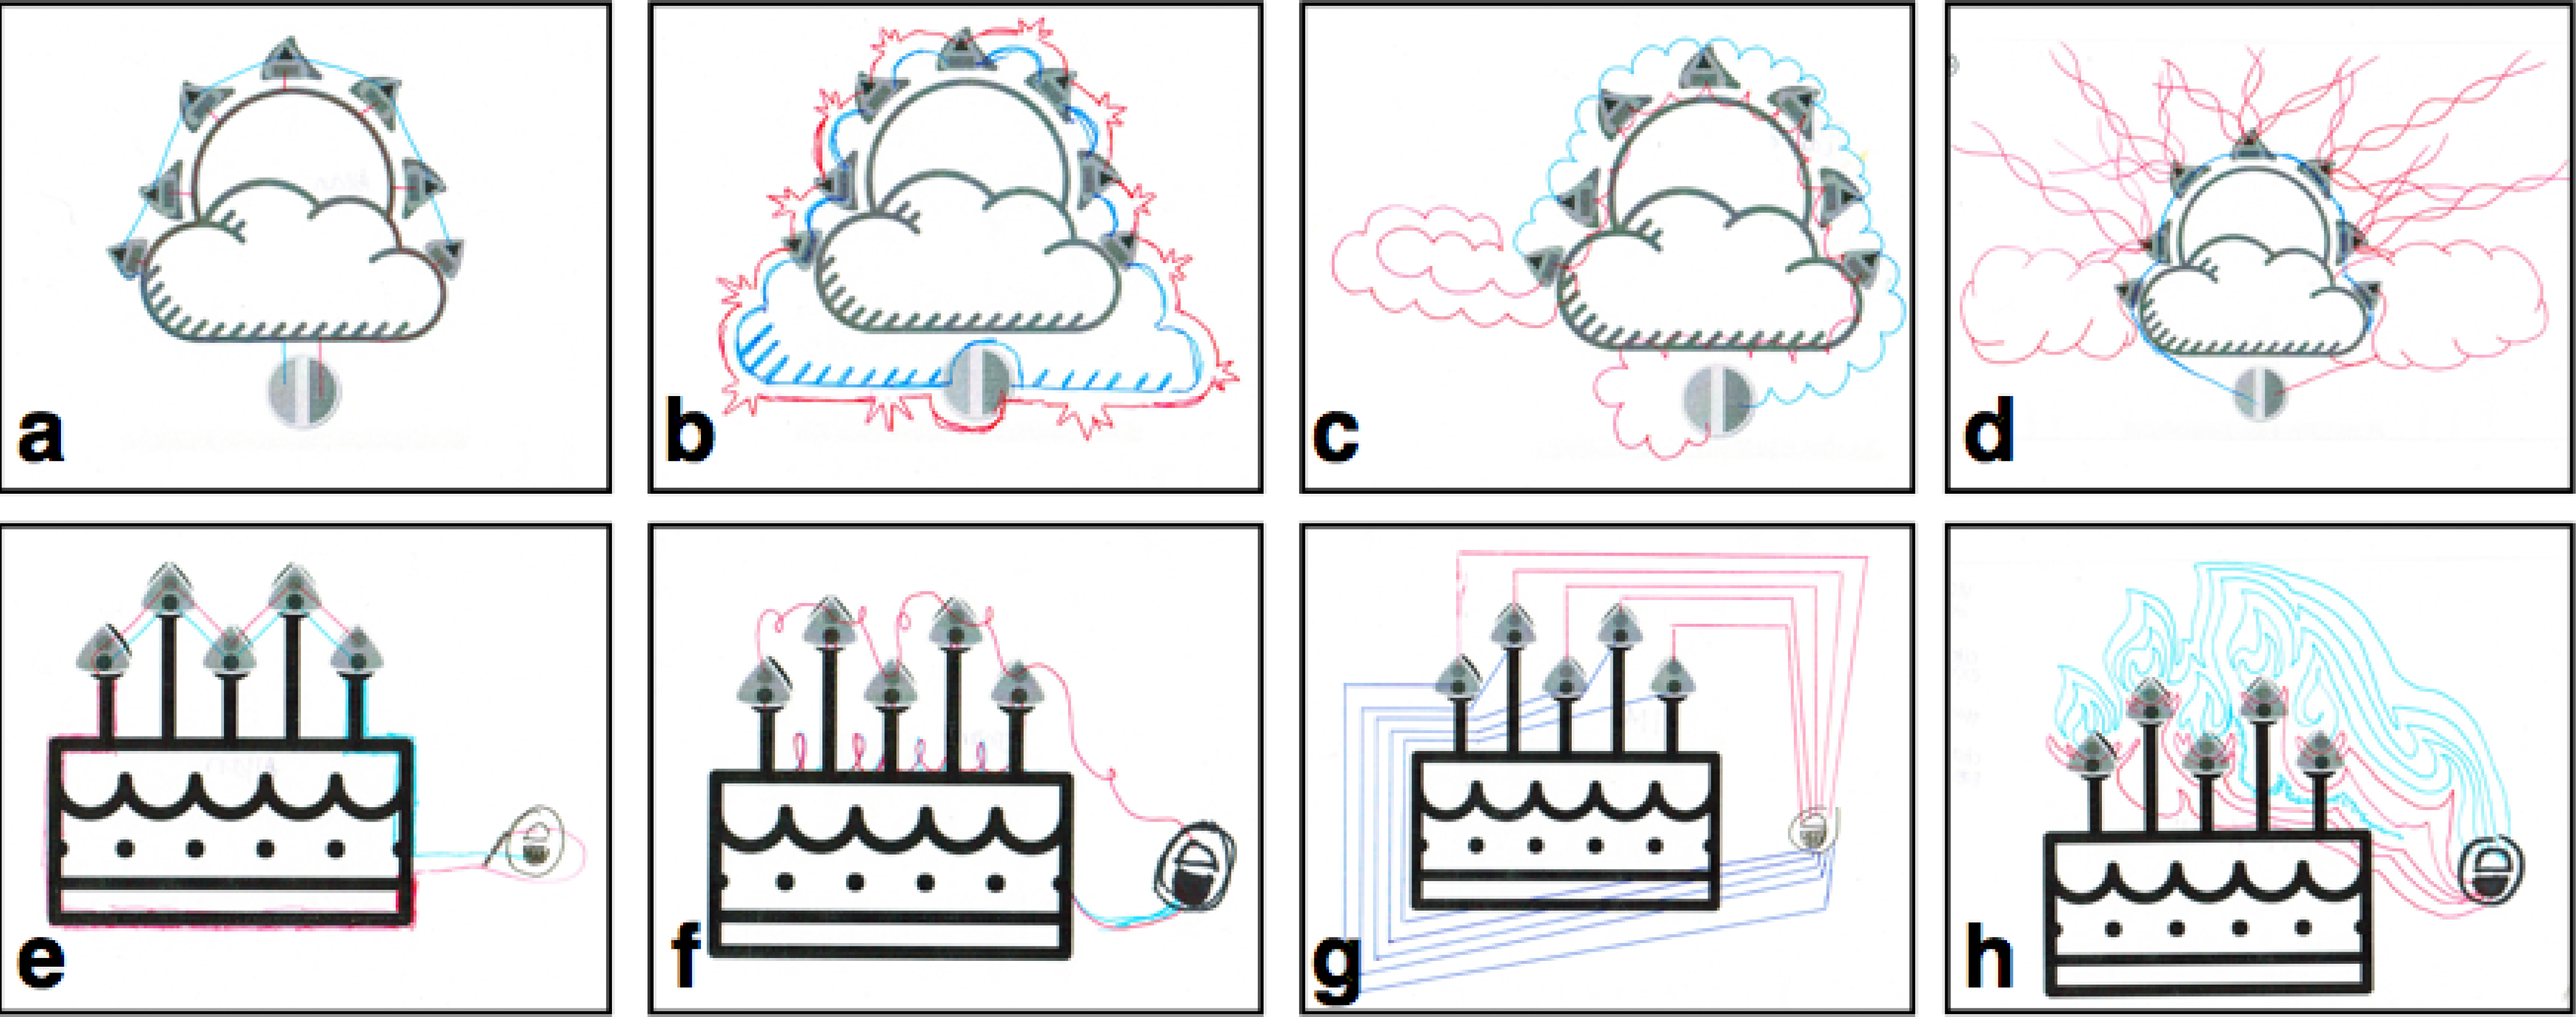
\includegraphics[width=1\columnwidth]{figures/Ellustrate_figures_formative_user_design}
  \caption{Formative user designs with pen and pencil}~\label{fig:formative_user_design}
  \vspace{-16pt}
\end{figure}

\section{Aesthetic Circuit Design Landscape}
The design of Aesthetic Circuits faces a few challenges since the requires careful considerations and balance of electrical, material, and visual aesthetic designs. There are four major features that a digital tool for aesthetic tool needs to include: 
\subsection{Freeform Circuit Drawing Tool}
The design of electrical traces that possess both electrical function and aesthetic value is possibility the most critical task in creating aesthetic circuits. In traditional circuit design tools, routing assistance is done in the form of auto trace - a algorithm driven process that determines the shortest and most efficient paths to connect electronic components on a given circuit board. Autotrace creates routing that minimizes board space and noise, but does not provide any aesthetic freedom. On the other hand, the design of aesthetic circuits, although needs to be functional, has less concern over board space and noise compared to a traditional electronic circuit board. Therefore, a digital tool for aesthetic circuit design needs to provide the freedom of creating artistic drawing but provide enough restrains to ensure electrical function at the same time.  Sketching circuits, especially when combine with visual design, can become a complex circuit routing puzzle. When the electronic components are placed in a nonlinear fashion, powering all of them without shorting the circuit or creating excessively long traces become difficult. In Qi el al, a paper template is provided to workshop participants to guide them in placement of the copper tape. While this method is highly effective in aiding participants in creating functional circuits, it limits creativity in visual design (cite).  Within Ellustrate, users are encouraged to explore and iterate different placements of electronics components and traces to optimize the balance between visual design and circuit functionality.

\subsection{Electronics and Materials Library}
Footprint and electronic properties (i.e. turn on voltage, maximum current) are important criteria in any circuit design. The understanding of these properties is essential to creating visually pleasing and functional circuit design. However, these vital information, which are readily available in any circuit design software (i.e. Eagle, Cadence, 123D Circuits), are not provided in any visual design software. This greatly limits ability of the designer to create a functional circuit and determine the visual incorporation of an electronic component footprint. In addition to the lack of electronic library, users that create physical circuits with nontraditional materials such as silver paint, graphite, and conductive thread face the difficulty fabricating traces with varying, uncharacterized, relatively high resistive materials. The problems that long, highly resistive trace often cause problems that are invisible to designers with little circuit design experience. 

\subsection{Fabrication and Debugging Guidance}
  The physical creation of the designed circuit is a difficult step in the process, as discovered in the Qi et al study, our expert survey, and formative user study. Solving hardware problems, which often requires probing using instruments in order to decompose the issue, can seem like a dark art to early circuit learners. In a workshop setting, guidance is provided to the participants to fabricate the circuit and debug any problems. However, in-person guidance is not easily scalable. Within Ellustrate, fabrication steps are provided in a step-by-step guideline, incorporating the modular fabrication process recommended by experts. Whereas debugging guidance, are provided in an expandable menu for users to access only when needed. 


 
\subsection{Electrical Validity}
  Circuit validation is a very large and complex field of study. In order to focus our contributions on circuit assistance design, we limit the scope of our circuit validation to deal with circuits with only LEDs, resistors, and batteries. The following design pattern can be extended to the more multi-faceted RLC (Resistance, Inductance, Capacitance) or circuits with integrated chips [Mellis].

  The most common task in electronic circuit design is the ability to connect components to sources of current. Most connections are modelled as perfect conductors, having a neglible resistance. As conductive materials enter this landscape, we encounter the need to represent the resistance or each connection (Equation \ref{eq:resistance}).


\section{Design Objectives}
  We synthesize the aesthetic circuit design landscape into the following objectives for a design tool. 
    
    \begin{itemize}
        \item Electrical validity: Circuits need to be electrically valid, prevent common mistakes.
        \item Legibility: Circuits need to be able to reach complex organizations, but remain legible for easy repair and sharing. 
        \item Fabricability: Circuits need to be makeable given a subset of materials. The tool needs to be aware of the materials available to the user. 
        \item Craft: The tool should incorporate a direct manipulation feel, with mechanical processes with constant interaction with the ``material" (Diderot) with a  ``continuum of states'' (McCullough 173)
        \item Expressivity: Users should be able to express their own creative styles and ideas. 
        \item Scaffolds: Designs should support users in creative thinking. 
    \end{itemize}
We use these objectives to guide the design Ellustrate, a web-based design tool that provides users with a suite of materials and components common to circuit sketching and guidance to design and fabricate a physical circuit.

\section{System Design}
The structure of Ellustrate follows the model-control-representation (physical and digital) (MCRpd)~\cite{ullmer2000emerging}. Ellustrate provides a digital representation of the physical system - the circuit design and the fabrication process - and allows users to iterate their design and modify their fabrication (i.e. debug). 

\section{Systems Details}
  % An overview of the tool can be seen in Figure 1. Ellustrate has three design phases \textendash Design, Fabricate, and Debug \textendash representing the three stages of physical circuit creation.
  % Within the Design cycle, users can freely explore and sketch circuits alongside the artwork that they wish to incorporate their electronics into, with Ellustrate Design providing visual clues for electrical connections and immediate feedback for electrical design errors.
  % Within Ellustrate Validate cycle, the digital tool not only checks for traditional mistakes such as misplaced ground connections, but also problems that are unique to sketched circuits, such as overly long and thin traces made with the relatively less conductive crafting materials (i.e. silver, graphite, conductive threads). After the circuit design is validated, Ellustrate Fabricate mode will provide users with step-by-step instructions on fabricating the circuit and debugging problems as they arise. 


    As an overview, the tool was designed on an Apple iPad Pro and Pencil, chosen to best emulate a pen and paper design environment.  Ellustrate exposes to users common vector editing operations; this was intended to expose a common vocabulary to our target users, who are expected to be familiar with the vector graphics. The tool is built using the paper.js vector graphics scripting framework~\cite{lehni_paperjs_2011} and follows noun-verb drawing application conventions (e.g. click on action icon, carry out action). At a high level, the tool allows users two operations: the ability to lay down components, and the ability to make marks representing different conductive materials.

    We chose to restrict vector operations to path drawing and affine transformations of objects. This was largely motivated by an interest in reducing the tool's complexity and exposing the hand-drawn line, as opposed to ``perfect'' machine curves, to achieve a sketching-with-pen feel.

    \subsection{SVG Representation}
    All elements on the canvas were encoded as Support Vector Graphics (SVG), where the hierarchical structure was used to denote the following encoding scheme by adding a prefix to element names:
    \begin{itemize}
        \item \textbf{Ellustrate Header} (\code{EL}): Used to demarcate the topmost layers of an SVG file that should be processed.
        \item \textbf{Material channels} (e.g. \code{SI} silver-ink) At this level, the type of material used to render marks is specified. This allows for these marks to be separated easily to aid with respective fabrication techniques (similar to CMYK channel separation for offset printing).
        \item \textbf{Components} (\code{CP}) Used to specify a set of conductive elements that conceptually belong together (e.g. LED, + / – terminals, footprint).
        \item \textbf{Elementary components} \code{C(N\textbar G\textbar V)(P\textbar B), NC, C(V\textbar G)TB}.
        The N\textbar G\textbar V selector designates the accepted polarity of the mark (neutral, ground, or powered). The P\textbar B selector specifies whether the conductive element is being modeled as a path or as a blob (closed path). The TB suffix is used to mark voltage sources.
    \end{itemize}

    This representation allows us to create custom components with accurate footprints and logic specification from off-the-shelf SVG editing software.We can readily export and import representations without affecting the operation of the artwork. 

    \subsection{Circuit representation}
      One of the largest challenges of extracting a circuit representation is the visual complexity from a simple sketch. Human visual-processing does an excellent job of grouping elements together, however if we extract a graph true-to-the-form of the digital sketch, we quickly surpass processing quotas for graph traversal for interactive applications (\~30ms). As such, we capture some of these visual Gestalt mechanisms in our graph extraction procedure using closeness as a grouping criteria to reduce the number of vertices in our graph (Figure \ref{fig:gestalt}). 

      \begin{figure}[t]
        \centering
        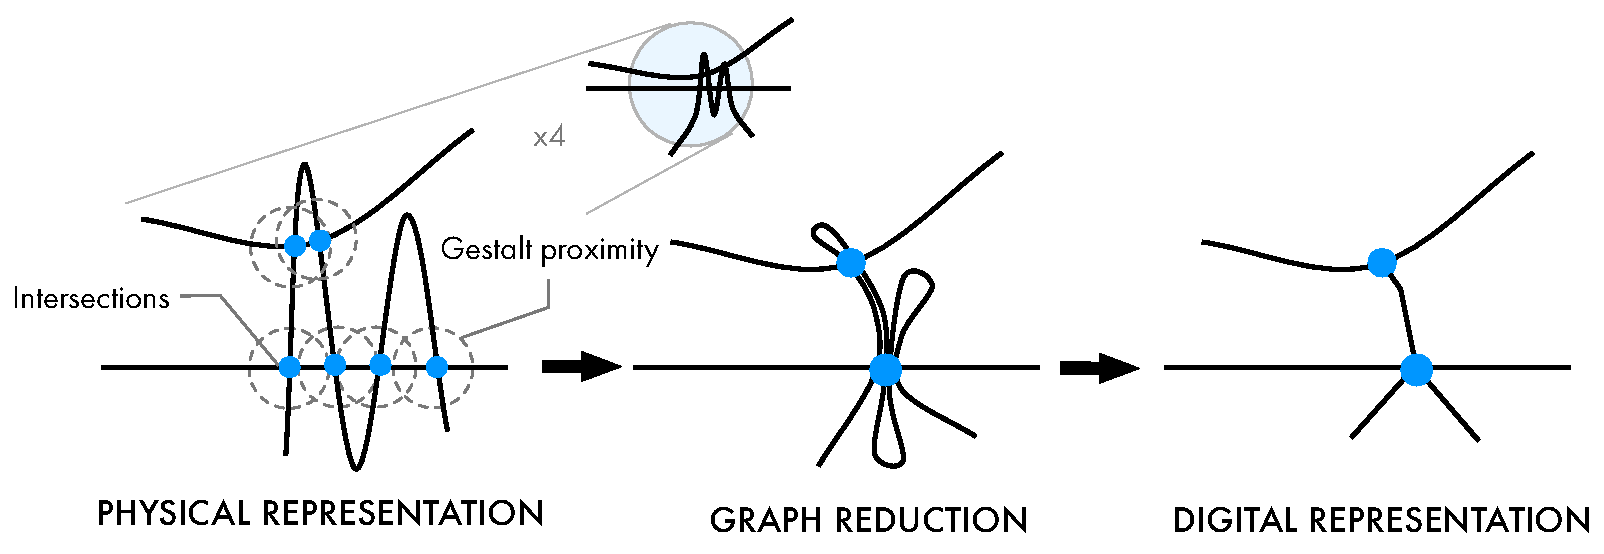
\includegraphics[width=1.0\columnwidth]{figures/gestalt.pdf}
        \caption{The complexity of a simple drawing, such as a scribble, adds significant computational complexity to a graph representation of a circuit. Ellustrate groups physically-close clusters of vertices together, reducing the complexity of the graph. }
        \label{fig:gestalt}
        \vspace{-16pt}
      \end{figure}

      \textit{Graph Extraction}.
      At the point when a user finishes drawing their Ellustrate circuit, we have an unconstrained number of SVG paths $p$. 
      Through a set of post-processing steps, we extract a graph representation of the circuit. 
      % (e.g. loops $\ell$, crosses)
      For each path intersection $s$ and self-intersection $t$, relevant paths are sliced at that intersection yielding $2(s + t)$ new paths. Intersections are disregarded if they occur at the start or end of the path, or if the two paths in question are collinear.
      For each blob intersection $b$, we draw a line from the blob center to the intersection point on the blob boundary yielding $b$ new paths.
      We then build an undirected $G$ using an adjacency list $\langle V, E \rangle$. We represent the start and end of each path as a vertex on the graph ($v = 4(s + t) + 2p + 2b $), and encode each vertex with its position on the canvas. An edge is defined as a connection where two vertices are collinear on a path or intersect another vertex; each edge is encoded with its material composition and cross-sectional area.
      % TOTAL VERTICES V = 4(s+t) + 2p + 2b
      % AFTER OPTIMIZATION V = s + t + b + 2p

      \textit{Optimization step}. We uses the physical proximity of each vertex to simplify the graph. Vertices which are close together are joined as shown in Figure \ref{fig:gestalt}) are joined and duplicate or self-referential edges are removed, reducing the total number of vertices by at most $3(s + t) + b$. This optimization reduces the number of vertices to $s + t + b + 2p$. To contextualize this information with respectice to sketching, this optimization allows us to work with a 86 vertex graph of the octopus in Figure \ref{fig:teaser}a (b = 32, s = 9, t = 17, p = 14) compared to a 196 vertex graph.

      
      Once this graph is extracted, we use breadth-first traversal to enumerate all paths between two points. In order to provide a more accurate model of conductivity for each of these paths, we derive a model from a set of basic electronic rules. Sheet resistance $S_r$ is the measure of resistance of thin films with uniform thickness; conductivity is modeled as the ratio of cross-sectional area and the length of the path. Thus, a path consists of a collection of edges $E$, where each edge $e$ has an associated material sheet resistivity $\rho_e$ and a sheet thickness $t_e$, which is simplified to sheet resistance $R_s = \frac{\rho_e}{t_e}$. We derive the resistance $R$ of a set of edges $E$ as:
        \begin{equation}
            R =  \sum^{E}_e R_s \int_{i=0}^{n}  \frac{1}{w_i} dl
        \label{eq:resistance}
        \end{equation}
      where $n$ is the euclidean length of an edge, and $w_i$ is the width of the path at offset $i$. Under this model, a uniform line \SI{2}{\milli\metre} thick and \SI{20}{\milli\metre} in length made with silver ink ($R_s = 0.5$) has a resistance of \SI{5}{\ohm} whereas a similar mark made with conductive thread (W = \SI{15}{\micro\metre}, $R_s = 2400$) has a resistance of \SI{1.8}{\ohm}.

    \begin{figure}[t]
    \centering
    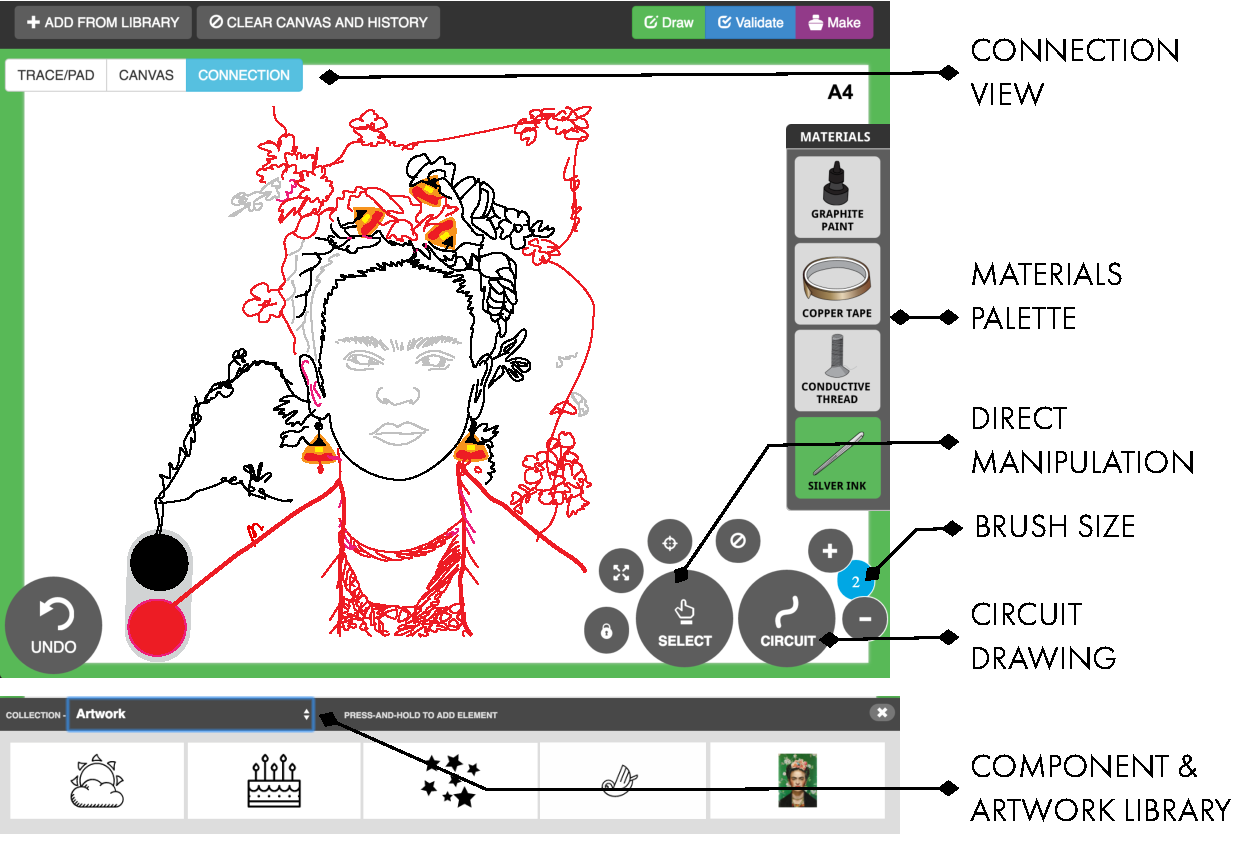
\includegraphics[width=1.0\columnwidth]{figures/designtool.pdf}
    \caption{Ellustrate design tool. }
    \label{fig:design_tool}
    \vspace{-16pt}
    \end{figure}
    
\section{Digital Design Tool}
    Ellustrate aims to alter the circuit aesthetic to allow for more expressive design and fabrication of circuits, balancing visual design with circuit constraints. In this section we detail common concerns of traditional circuit design, and how Ellustrate approaches these circuit constraints.

    \subsubsection{Preventing shorts}
    These connections must have an adequate resistance to prevent electrical shorts. As such, paths that originate from the voltage source (\nt{V+}) cannot make contact with paths connected to ground (\nt{GND}).

    In order to support this concern, we color-code paths, pads, and other conductive elements with different polarities as either red (positive), black (negative), or gray(neutral) and establish the following visual rule:
    \\
    \\
    \noindent\fbox{%
    \parbox{0.465\textwidth}{%
       \textbf{Visual Rule I.}
       Connections can only be made from/to similarly-colored (i.e. red\textbar red) elements or from/to neutral elements (i.e. gray).
        }%
    }
    \\
    \\
\begin{figure}[h]
\centering
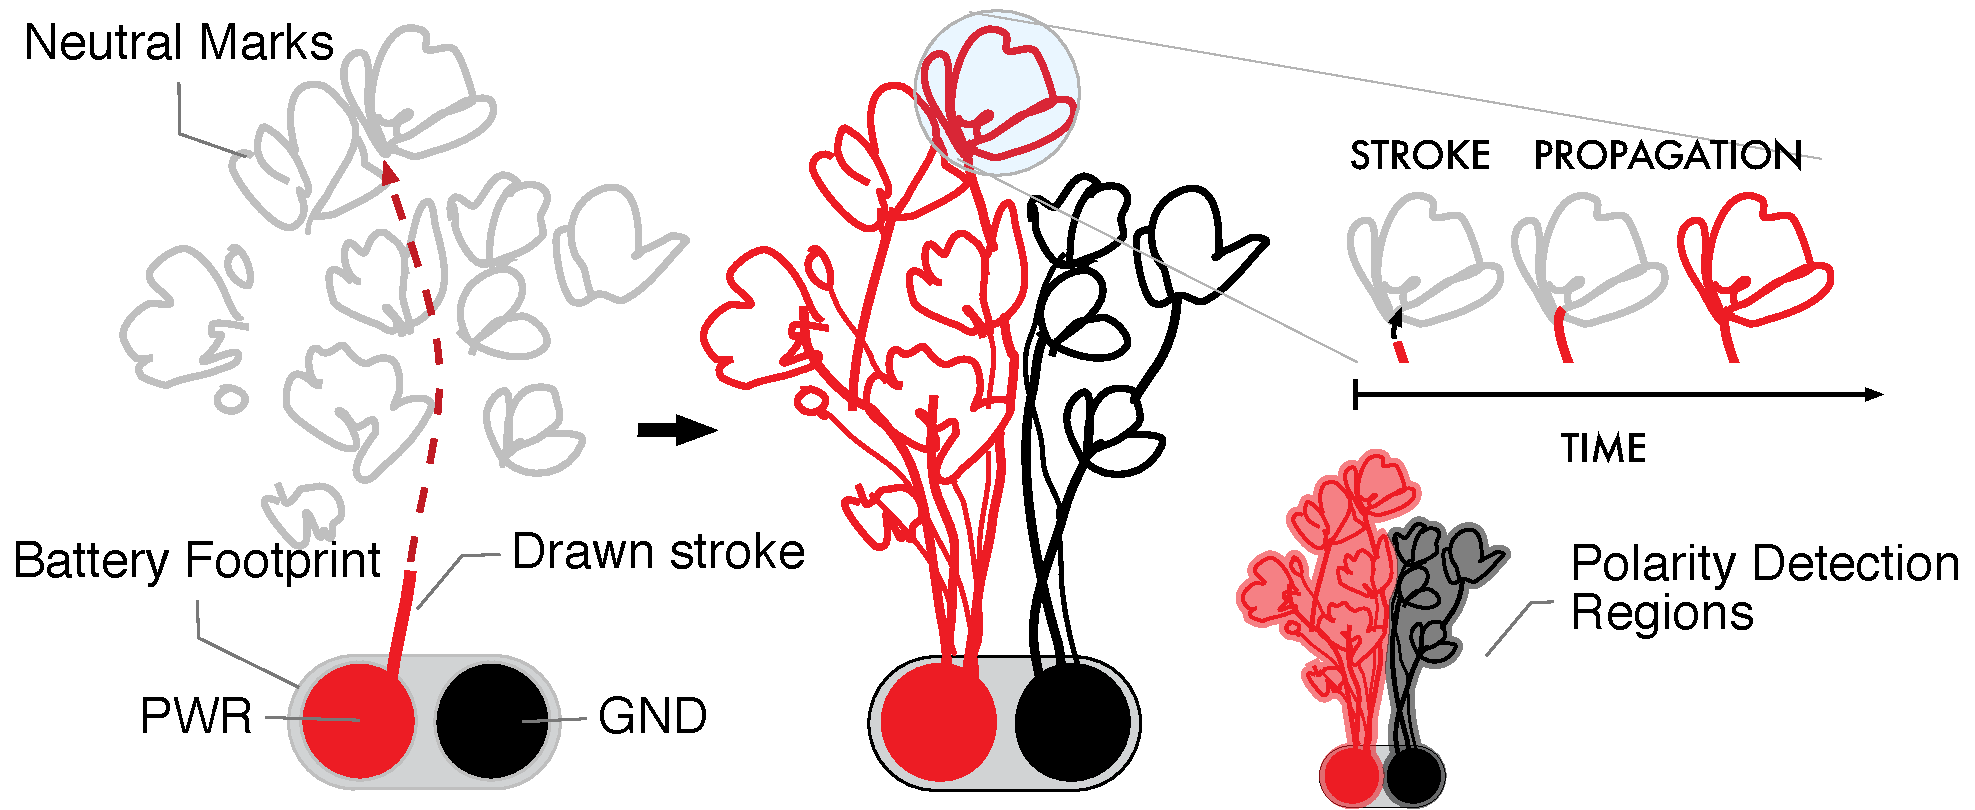
\includegraphics[width=1.0\columnwidth]{figures/propagation.pdf}
\caption{On intersection with a neutral components, path polarities update. This allows for users to design elements and then electrically incorporate them. }
\label{fig:propagation}
\end{figure}
    Should such elements cross, our tool signals offending paths to the user and are removed. If a polar connection makes contact with a neutral element, the polarity is propagated to all elements touching the neutral element (Figure \ref{fig:propagation}). This ensures that at any given time, no shorts exist within a circuit design.



    \noindent\fbox{%
    \parbox{0.465\textwidth}{%
       \textbf{Visual Rule II.}
       All polar elements need to be connected to its respective battery pad.
        }%
    }
    
    
    \subsection{Legibility}
        Glow relevant traces as needed.
        Connections view.
        Strip traces and show connections.

\section{Fabrication Tool}
    Once a circuit has passed digital validation, we provide a set of design-specific fabrication instructions and schematics. For clarity, we describe the fabrication system with respect to silver-ink as the conductive material, but detail which portions of this process is portable to other materials. 

    \subsection{Design schematics}
        The Ellustrate design tool outputs a to-scale version of the circuit as an SVG file, which is then printed or transfered onto a circuit substrate (e.g. paper, tattoo paper, etc..). Conductive paths are denoted with dashed magenta lines to indicate where traces should be drawn.
        Each component footprint is outlined and labeled. Lastly, a printable bill-of-materials (BOM) is produced to aid with planning and record-keeping.

    \subsection{Design-specific fabrication instructions}
        To prevent common fabrication mistakes and to layout an easy-to-debug circuit, Ellustrate generates instructions that encourage modular fabrication. To decompose the circuit graph, we query our scene graph for all LEDs on the canvas. We then extract the shortest (least resistant) path to power (\code{CVTB}) and to ground (\code{CGTB}) for each LED, and order these paths by length, which we will term branches. By fabricating each of these branches in sequence, a user can modularly test each branch in isolation. We arrived at the following fabrication procedure for circuit building through several pilot iterations with target users. For each instruction, our tool highlighted relevant parts of traces and components. For instructions that required the use of a multimeter (\code{MULT}), our tool displayed an image of the multimeter with the correct dial placement and visually-annotated where multimeter probes should be placed on the circuit. 

        Each instruction set begins with affixing a power source to the circuit. Since a power source is needed to test each branch, we keep it affixed in order to remove this variable from needing to be debugged. 
        \begin{enumerate}
              \item {[}Draw{]} the initial portion of all traces originating from the battery. [Dry].
              \item Add the battery.
              \item Power Check: For each power-ground path, check that a voltage greater than 3.3 V is observed. (\code{MULT})
        \end{enumerate}

        The instruction set is then appended with branch fabrication steps. Certain fabrication are set to require confirmation feedback from the user.In the case of a negative confirmation, a debugging step is added to the instruction set and removed once resolved. Certain material-specific instruction can be generated to aid with fabrication. For instance, in the case of silver-ink, it is unpredicatable as to how long it takes the ink to dry. Wet ink has a higher resistance and might impede circuit function. Utilizing our modeled conductivity, we can provide users an idea of what type of resistance they should expect, as well as a simple countdown timer to take the guesswork out of dried ink.  
          \begin{enumerate}  
              \item {[}Draw{]} both positive and negative traces in branch, [dry].
              \item Check resistance of positive trace is about 2X ohm. If not, [dry, widen, continuity]. (\code{MULT})
              \item Check resistance of negative trace is about 2X ohm. If not, [dry, widen, continuity]. (\code{MULT})
              \item Place LED, pay attention to orientation; [handling].
              \item Check if LED turns on. If not, [press down, goto]
          \end{enumerate}
        Similarly instruction are substituted or added for using and debugging different materials, such as:
        \begin{itemize}   
          \item {[}Dry{]} Material-specific drying times (graphite ink takes longer to dry than silver ink). 
          \item {[}Widen{]} Thickening traces for higher resistance. 
          \item {[}Handling{]} For circuit stickers, ensure that adhesive pads are ink-free, avoid removing stickers from paper, do not touch adhesive side. Copper tarnishes from hand oils; wash your hands. 
          \item {[} Continuity{]} A continuity issue results when a trace is not fabricated correctly; a break in this trace will result in an interrupted connection preventing the flow of electricity. Use the multimeter in continuity mode and place both probes at [start]. Move one probe towards [end], checking that the trace is continuous (beep throughout).  
          % \item {[} Polarity Check {]} A user is provided with this template circuit which connects two traces to the a battery. A user can place the component of interest, such as an LED, and check the polarity of the component by placing it on the traces and observing changes in behavior. Should a user experience a non-working LED, they are encouraged to verify that the orientation of the LED be correct. Although we don't foresee these issues being of major concern since LEDs are housed in perceptually-identifiable packages, we recognize polarity being a common issue and provide a simple tool to address it.
          \item For conductive thread, larger patches need to be sewn for connection terminals; single strands may not be conductive enough. 
          \item For copper tape, a common debugging technique is to lay additional copper over problem areas. A rule of thumb is to use continuous pieces of tape. To reduce connection errors and make copper tape more aesthetic, one can use a bone knife to press-down and smooth copper tape. 
        \end{itemize}

\section{EVALUATION}
    Here we describe an overview of our formal user study. The goal of this study was to conduct a usability evaluation of the tool, specifically observing at how circuit design contraints influence the visual aesthetic and how fabrication assistance influences agency. 

\subsection{Participants}
    We recruited 10 participants (avg. 28 years, 7F, 3M) well-versed in visual design, but with no prior experience with circuit design. Proficiency was self-reported in a preliminary survey. Participants were recruited from a mailing list of Architecture, Art, and Design students at our institution and from the surrounding community via Craigslist.

\subsection{Materials}
    We constrained our evaluation to a single circuit building material --- silver ink was chosen due to it's user-friendly pen form factor to have analogous tangible input with the Apple Pencil. For the study, our electronics library was constrained to fixed set of finger-sized manipulatives: 5 Chibitronics LED stickers, and a single CR2032 coin-cell battery.We also exposed a set of SVG graphics with different layout compositions (figurative, linear, radial, and random placement) in order to evaluate how users navigate circuit rules with spatial constraints. 

\subsection{Study Design}

    Each participant was invited to individually meet with us in our studio space. Participants were paid \$20/hr; each session lasted two hours and consisted of a warm-up tutorial, a digital design task, a physical hand-fabrication task. We also conducted interviews before and after each session. Participants were also asked to reflect out-loud their reflections on tools and design process, specifically vocalizing their design choices and shifts, as they went through the workshop. Due to the visual complexity of the circuits, the experimenters aided with interface and fabrication issues when they arose. We report such occurrences for future work to support a larger corpus of visual styles.
    
    \begin{figure}[h]
    \centering
      \includegraphics[width=1\columnwidth]{figures/Ellustrate_figures_Users_in_action}
      \caption{Users designing and fabricating their circuits with Ellustrate}~\label{fig:users-in-action}
      \vspace{-20pt}
    \end{figure}

    % power requirements
    \textit{Warmup}. We provided participants with relevant background information for understanding the primary concerns of circuit design and building. A brief introduction covered basic electrical design rules (e.g. connecting power and ground, avoiding shorts) and operation of equipment (drawing traces with a silver ink pen; checking resistance and voltage with a multimeter). Tutorial material was available as reference throughout the study. 

    \textit{Design Task}. Participants were then given a design task to design a circuit with any or all of the available materials for a period of 20 minutes. They were asked to design a circuit with five LED's in parallel, with at least one background artwork incorporated. A five LED's provide a reasonable level of routing and aesthetic difficulty to be solved within 20 minutes. Parallel circuits also tend to create more routing complexity in an aesthetic circuit and require more creative solutions. If there were issues, they were asked to attempt to fix and iterate on their circuit design using features provided within the tool. 

    \textit{Fabrication Task}. Once successfully validated, our system produced fabrication instructions. A to-scale schematic was printed. Users were asked to fabricate their circuits using five circuit sticker LED's. They were given 40 minutes to complete the task using fabrication and debugging instructions provided by the tool.  

    We asked participants to seperately rate their experience with the design tool and the fabrication tool using five-point semantically anchored Likert questions (1=Strongly Disagree, 5=Strongly Agree):
    \begin{itemize}
      \item \factor{Assistance (As)}: The tool helped my circuit [designing/fabricating] process.
      \item \factor{Pre-Agency (pA)}: I feel capable of [designing/fabricating] a circuit before using the tool.
      \item \factor{Post-Agency with Tool (ApT)}: I feel capable of [designing/fabricating] future circuits with the tool.
      \item \factor{Post-Agency without Tool (Ap)}: I feel capable of [designing/fabricating] future circuits without the tool.
    \end{itemize}
    In particular, \factor{ApT} describes the experience of designing a circuit with Ellustrate, while \factor{Ap} generalizes to how Ellustrate may serve as a tool that enables lasting skills in aesthetic electronics design and fabrication.

\section{Results}
All participants successfully completed their designs; some designs are represented here in Figure \ref{fig:user-artwork}. 
We first report quantitative results and then discuss interview responses in the context of specific observations and insights from the study.

\begin{figure}[t]
\centering
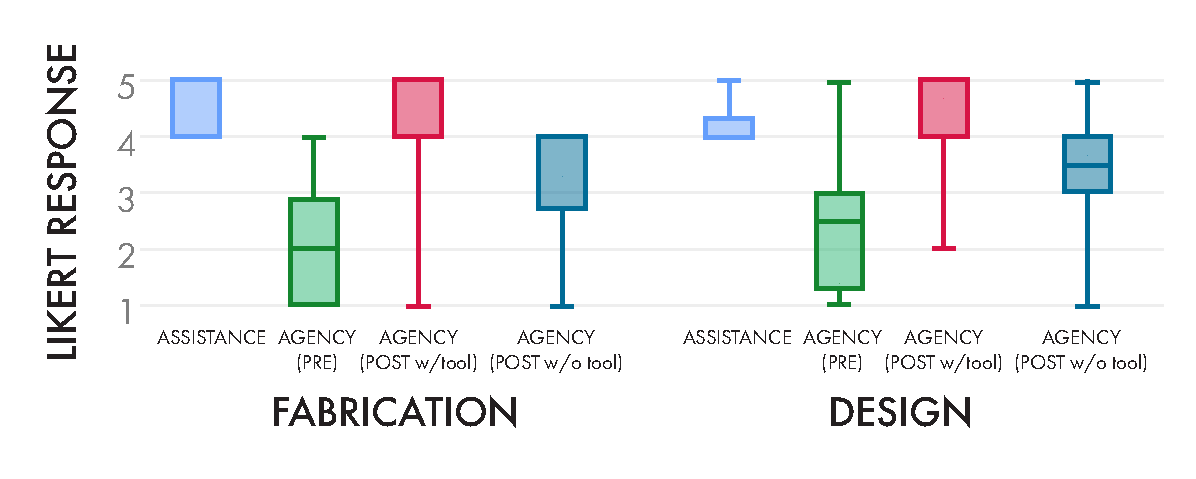
\includegraphics[width=1.0\columnwidth]{charts/boxplots_quant.pdf}
\caption{Tool evaluation responses. Overall, participants reported feeling more agency to create their own circuits after using Ellustrate, and felt that the tool assisted them with both design and fabrication.}
\label{fig:fab_tool_results}
\vspace{-20pt}
\end{figure}

  At the onset, participants expressed uncertainty and apprehension when asked to produce a visual circuit design (\factor{A} $2.4 \pm 1.26$), specifically noting \cesar{the large amount of information presented to them created a large cognitive block to what they were going to draw}
  \begin{myquote}
   \vspace{-2pt}
    \participant{Participant \#???}:
    \quoted{ I wish I could say I could make that circuit. But with all those constraints, its hard for me to even think creatively. I'd rather try to make a simple circuit, get that working, and alter my design little by little from my known threshold of skill.}
    \vspace{-2pt}
  \end{myquote}
 % \cesar{Jasper: verify the below} \jasper{No support found :(}
  All participants reported feeling that the design interface assisted them in creating the design (\factor{A} $4.2 \pm 0.42$). They felt the assistance non-intruding, citing the visual rules as fun and interesting. 
%   Many participants expressed that they wanted to design using the black and red as design elements in their visual compositions and noted that the constraint of color opened their compositions to be more explorative. 
%     \begin{myquote}
%   \vspace{-2pt}
%     \participant{Participant \#???}:
%     \quoted{ I know that the red and black are electrically important, but I just like how they look in my composition.}
%     \vspace{-2pt}
%   \end{myquote}
%   Participants expressed a heightened caution from accidentally overlapping colored paths; few participants triggered the warning. Those who did expressed surprise and immediate recognition of their error. 
%   \begin{myquote}
%   \vspace{-2pt}
%     \participant{Participant \#???}:
%     \quoted{ I dozed off, but its okay. I know exactly what I did wrong; I realize I have to keep these elements on separate sides of the page. It causes my to think and plan, but I find that interesting and stimulating.}
%     \vspace{-2pt}
%   \end{myquote}
  Many felt the tool empowered them to visually create their own circuits (\factor{ApT} $4.0 \pm 1.22$). Several expressed agency to even create designs without the tool (\factor{Ap} of $3.4 \pm 1.27$), noting the simple coloring scheme as the most valuable in aiding their visual design practice.

  \cesar{Some note about validation and them going back to fix designs. Insert fatal errors here. People are too *** creative.... Number of vertices on a design was v= 10000000, compared to its stale circuit equivalent of v=8, e=30. Optimization steps need to be taken to prune the electrical tree during drawing time.}

  Participants expressed a much larger difference with the fabrication tool. Although in a familiar form factor, users still expressed hesitation (\factor{pA} $2.1 \pm 1.2$) especially with regards to understanding when to use the multimeter. The fabrication tool provided for them with much needed guidance; participants felt highly assisted with the tool \factor{A} $4.4 \pm 0.52$. Many expressed that their own construction patterns were completely different from the tool's suggestions.
  \begin{myquote}
   \vspace{-2pt}
    \participant{Participant \#???}:
    \quoted{I had no idea where to begin! As I was doing the steps, I realize I would have gone about this totally differently. }
    \vspace{-2pt}
  \end{myquote}
%   The most common intended fabrication process was laying out the traces, then adding the components. 
%   However, as they moved through the fabrication steps, all participants detected the pattern and after practice with the modular decomposition, likened it to a ritual, mechanic repetition of the hands that they experience when in their respective crafts.
%   \begin{myquote}
%   \vspace{-2pt}
%     \participant{Participant \#???}:
%     \quoted{I started seeing the pattern and the intention behind the steps. Putting the battery first allows me to not have to worry about power as a variable. Drawing modularly the electric lines makes it much more likely that I will succeed.}
%     \vspace{-2pt}
%   \end{myquote}
%   Many reported the modular lighting of LEDs as motivation to keep on continuing; there was a general consensus that more fanfare was needed.
  Notably, the tool segmented the fabrication steps into modules, where an additional LED would light up at the end of each module. For many, this was not only incentive to continue on with their design, but also a source of confidence.
  
  \begin{myquote}
   \vspace{-2pt}
    \participant{Participant \#???}:
    \quoted{ Once I got the first light to turn on, I knew I could complete the circuit. Each light was like a little treat. Upon running into a problem, I felt confident that I could solve the issue.}
    \vspace{-2pt}
  \end{myquote}
  
  At the same time, we noted differences within the role of the tool. One participant found the construction initially useful, but once they learned the process they felt that it was simple to replicate on their own (\factor{Ap} $3.3 \pm 1.3$).   They noted that the multimeter operation was intimidating, but after using it, they felt it was greatly helped in revealing what was happening with the circuit. They expressed an interest to be able to ``dive deeper'' into the reasoning and the logic behind the steps and how the internal circuit is operating. The most valuable feature of the fabrication tool was the visual highlighting of paths and a feeling of being guaranteed a success (\factor{ApT} $4 \pm 1.7$). 

  \begin{myquote}
   \vspace{-2pt}
    \participant{Participant \#???}:
    \quoted{ Whoa. I realize my circuit is super complex. I'd hate to spend all this time drawing my detailed illustration and not know which line is important to the circuit. When I clicked this [highlighting of the path], it takes away that need for me to visually trace the path to the battery. }
    \vspace{-2pt}
  \end{myquote}
  % Given an overall \factor{AGENCY PRE-} of , we observed an increase in agency after using the tool with an \factor{AGENCY POST- (WITH TOOL)} of $4 \pm 1.73$ and an 
% 
  % In both the fabrication and design steps, we observe strong increases in both agency metrics, suggesting that the tool successfully enabled users with various backgrounds in circuit design to create circuits with a high degree of agency.
  
  The qualitative data begin to describe more general user experiences with the tool. Below, we extract some notable trends in how participants chose to navigate a constrained design space. 
\subsection{Aesthetic and Electrical Planning}
  As Ellustrate was designed to facilitate the visual aesthetics of circuits, it was important to observe how users balanced electrical requirements, electronic layout, and  aesthetic considerations. Notably, ease of routing was a big factor that drove many designs, which was to be expected for people with no background in circuit design. However, the way in which participants reacted to routing issues varied.
  
  \participant{Participant \#72}: 
  \quoted{I thought grouping the LEDs in a geometrically symmetric way, they would be easier to route.}
  
  
  \participant{Participant \#335}: 
  \quoted{I didn't understand that the wires don't need to be hidden. Now that I know, I am going to make them into twinkle lights that tie to the LED.}

  We distinguished three types of marks that characterize how participants navigated around circuit rules to create their visual design, as detailed below:
  
  \begin{figure}[h]
\centering
  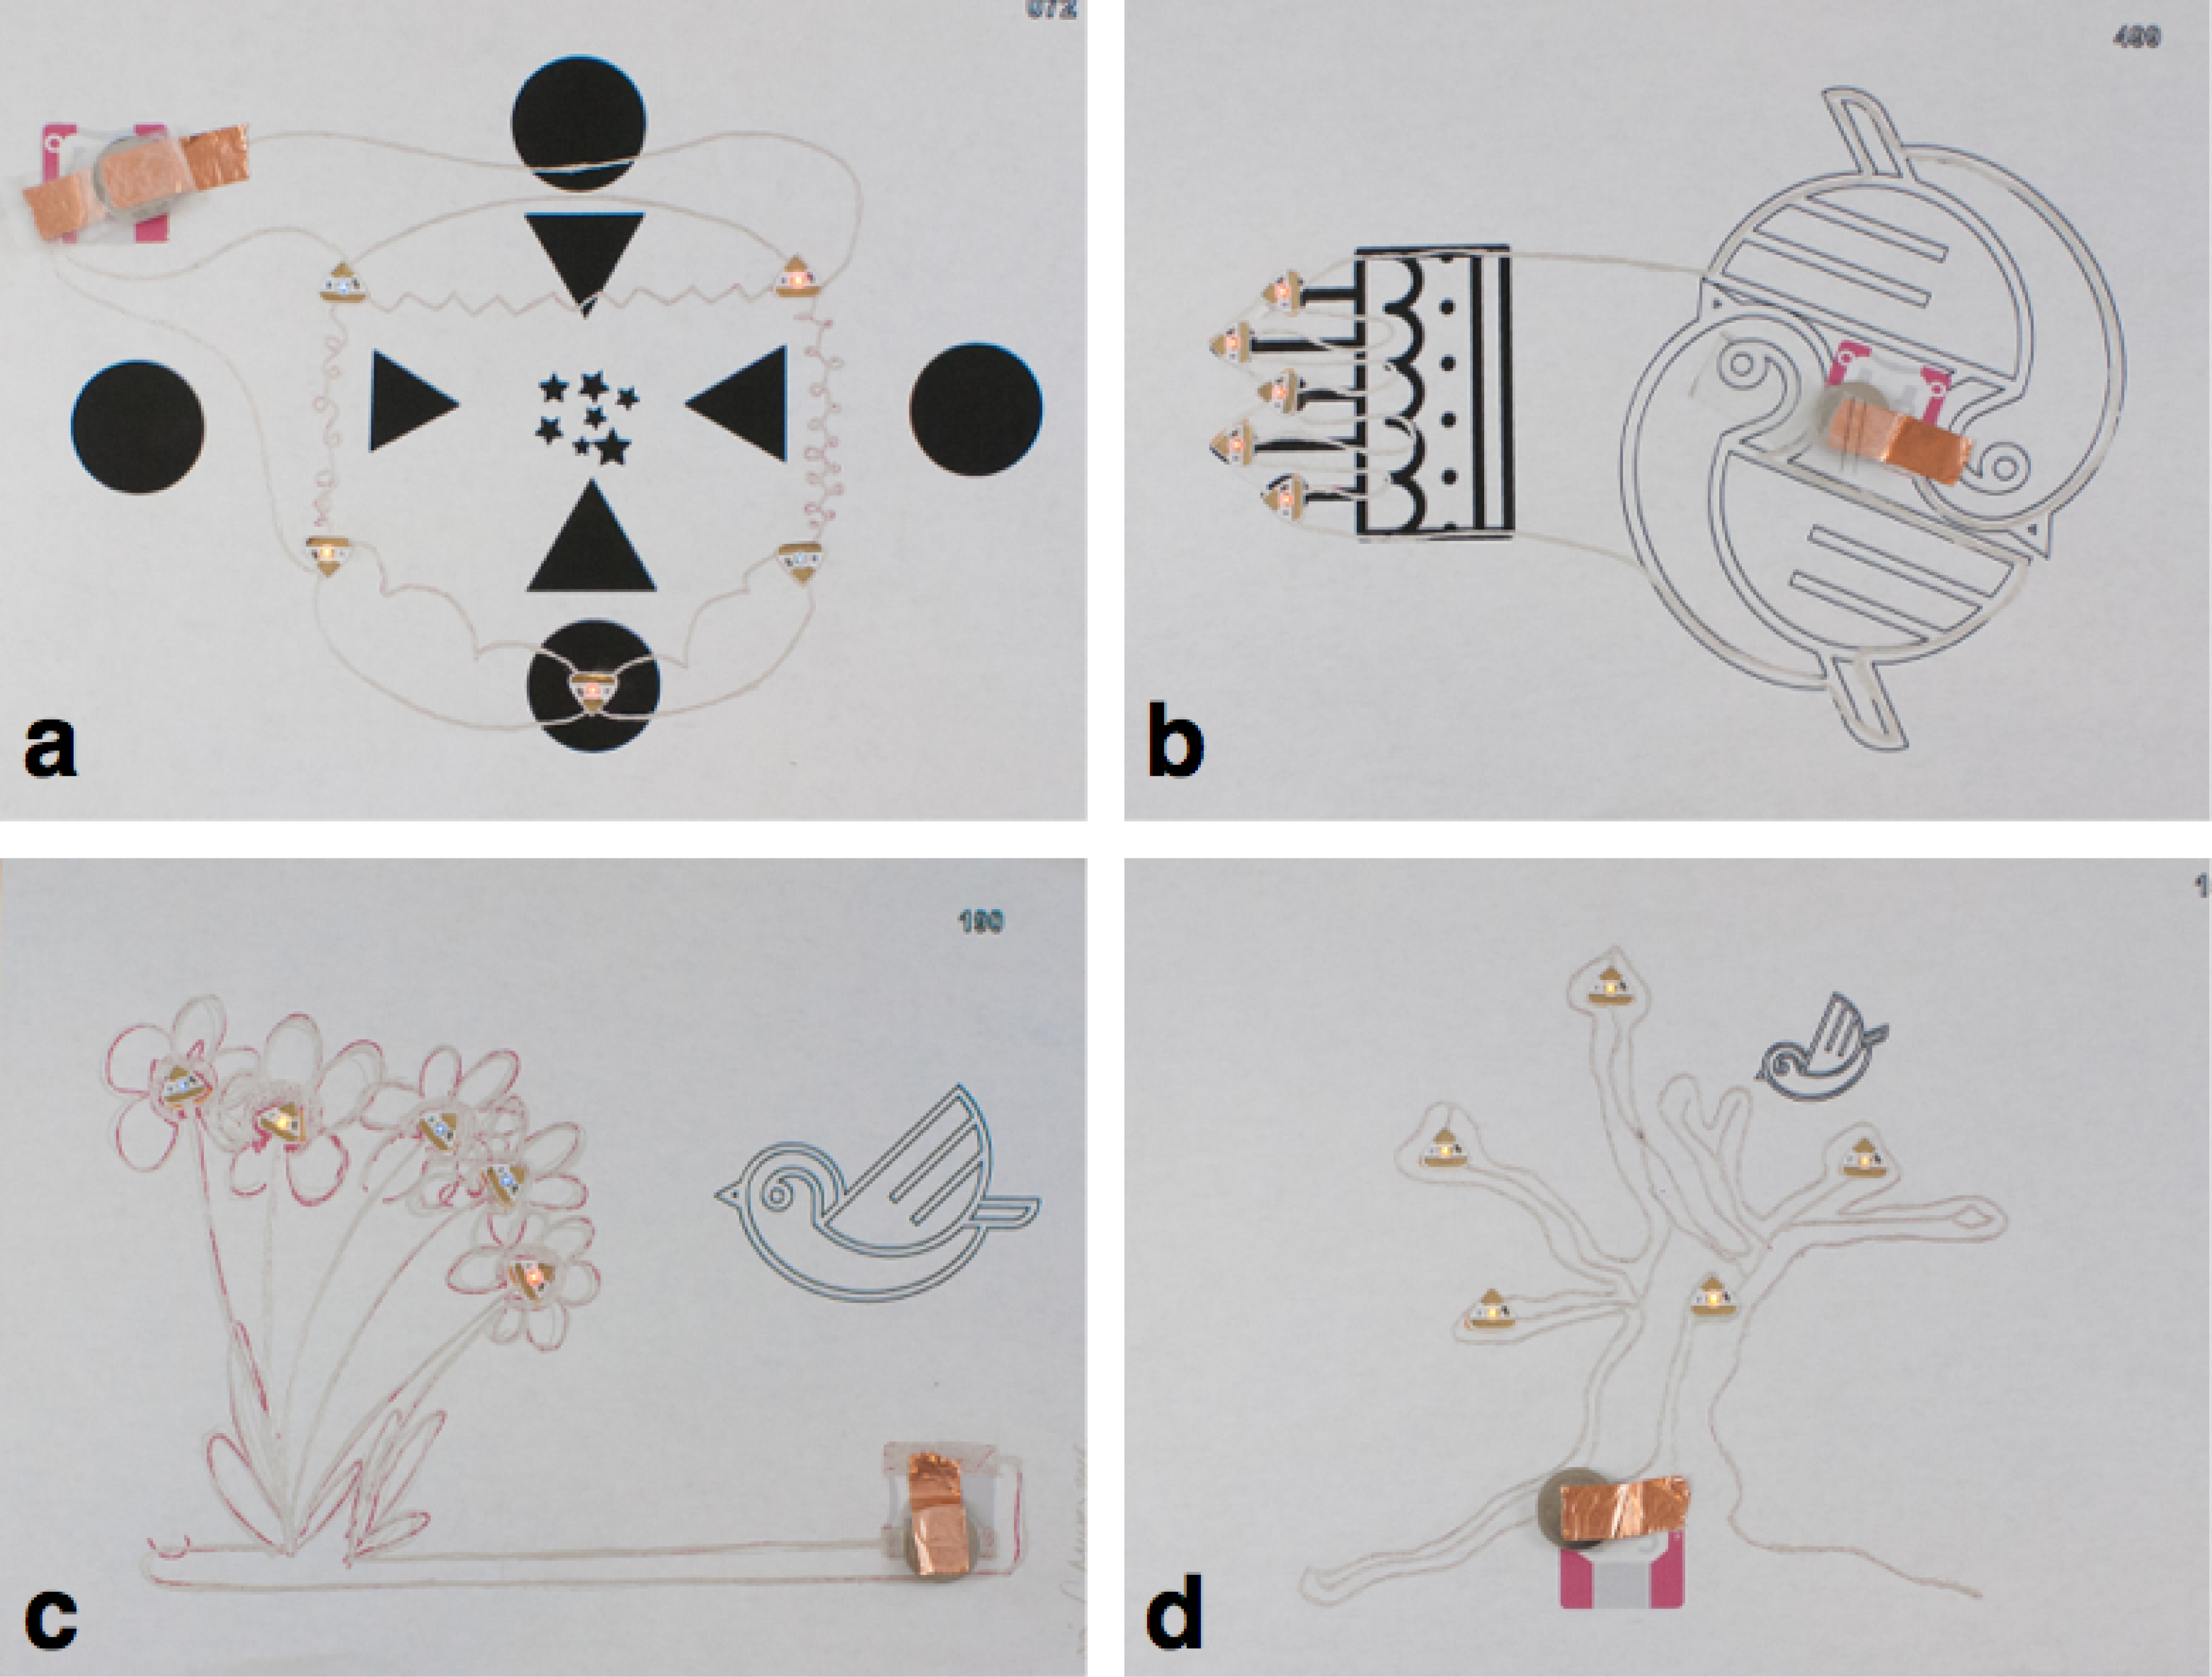
\includegraphics[width=1\columnwidth]{figures/Ellustrate_figures_Users_artwork}
  \caption{\jasper{Retake this figure to match refs below}Sketched circuits made by users}~\label{fig:user-artwork}
  \vspace{-20pt}
\end{figure}

  \textbf{Functionalist:} While all participants tended to position LED footprints in semiotically relevant places (e.g. matching the triangular shape of the LED footprint with the candle flames), participants with more prior circuit experience were more constrained to a functionalist aesthetic, drawing lines that minimized distance and distractors. Often, they drew over the design in search of a shortest path. These participants desired the ability to mask portions of the line using a paper mask.


  \textbf{Mimetic:}
  These designs adhere to the design language of the existing SVG, but that are not completely constrained to shortest paths. A common pattern was using the contour of the sun as aesthetic scaffolding to connect LEDs positioned in the rays of the sun. A more extreme case is how Figure \ref{fig:user-artwork}b displays mimicking the texture of the star field SVG. Their design features additional stars that she drew, and this emulates the existing texturing of the SVG. In these scenarios, because participans mimic the existing design language, the choice of SVG highly influences participants' final designs.
  
  \textbf{Constructive:} In contrast to functionalist and mimetic lines, some participants drew objects wholly outside of existing SVG scaffolding. Notably, Figure \ref{fig:user-artwork}c has the main circuit as a tree, given only the bird SVG. Interestingly, the participant drew a graphic correspondence between then bird and tree branches, as well as a semantic correspondence with branching wire (a concept from electrical engineering) the tree branches.

  \begin{myquote}
  \vspace{-2pt}
    \participant{Participant \#156}:
    \quoted{I thought of something where I can branch out the wires, and I thought ``bird and branches.''}
    \vspace{-2pt}
  \end{myquote}
  
  \textbf{Symbolic:} Some participants used to tool to go beyond lines as a means of connecting wires, but instead as a means of ascribing meaning to lines. Figure \ref{fig:user-artwork}d illustrates this with a ``yin-yang'' formed by the two birds. Other traces and footprints then conform to the meaning established by the birds. With metaphorical lines, participants satisfied not just two criteria: a) functional requirements of a trace in a circuit and b) aesthetic considerations, but also developed a ``language'' or a system of meaning based on the traces.
  %This is semiotics, the emergence of artistic talent in a new circuit-drawing medium. 
  This is the building blocks of narrative or \textit{electronic storytelling}, which we detail further below.
 

\section{Observations and Insights}
  We report observations of subjects experience designing and fabricating aesthetic circuits and draw design principles for the design of smart design and fabrication tools. 
  
  \subsection{Translation Between Digital and Physcial Mental Models}
  Most participants came in with a basic understanding of electricity. Although our water metaphor introduction was our grounding mental model in our introduction, we noted several amalgamations of previously held mental models. Most prevalent was a ``two-pronged plug'' model, where each LED was viewed as a lightbulb with a two-pronged directional plug and the battery as a socket. We found that participants with no circuit experience relied heavily on the interface mechanisms used to convey circuit rules, adopting the visual vocabulary of the interface (e.g. ``red and black'' vs. ``positive and negative''. The construction of their mental models were so heavily reliant on the interface for some, that some participants reported a mental color synesthesia whereby subjects memorized the coloring of the traces in the digital design phase, and held that representation as they worked on their silver ink fabrication. This observation shows tremendous opportunity to use digital representations to influence how users perceive and operate in the physical world and the large ethical power of interface designers to provide a grounded model from best practices. 

  \subsection{Step-by-step Fabrication Can Overconstrain}
  Although constraints are well-documented in HCI research to improve creative thinking, we found the constraint of an instruction set during the physical fabrication of participant circuits often inhibited participant's ability to develop a creative mental model for the circuit. The step-by-step or ``checklist'' style fabrication pipeline was the primary reason why users reported low agency (\factor{Ap, ApT}) after completing the task with the tool. In particular, participants who self-identified as artists found that the fabrication tool restricted their sense of creativity.
  % These participants reported a lower average \factor{AGENCY POST- (WITH TOOL)} of $1$, even though they reported an average \factor{AGENCY POST- (WITHOUT TOOL)} of $4$. When asked about what they disliked about the fabrication tool, both reported a reduced sense of agency in the artistic sense due to the constraints interface's pipeline.
  \begin{myquote}
   \vspace{-2pt}
    \participant{Participant \#159}:
    \quoted{There should be more options for shapes, and color as well as a grid. Validate mode is hard to get to... I kept forgetting to check the steps to complete them. It didn't exactly click for me.}
    \vspace{-2pt}
  \end{myquote}
%   These participants felt more empowered without the tool, wanted to generate their own methods of making versus fall into the regimen of the machine. \jasper{However, the artists didn't realize that they totally couldn't do anything without the tool} The underscores that pipeline processes did not adhere to creative thinking in the holistic design process.
  While these participants reported feeling more empowered without the tool, we must also consider consider that the constraints of the step-by-step also allowed participants with less circuit knowledge to implement a creative designs without worrying about implementation details.
  
  \subsection{Incentivizing Tinkering and Debugging}
  Because the step by step instructions created a guaranteed safety net, they were able to disregard the interface's steps and instead began to make design decisions based off of their own intuition. Once participants gained proficiency with the tool, they developed their own behaviors independent of the step-by-step instructions, such as blowing on the conductive ink while it was drying. Some commented that they thought the allotted waiting time of 60 seconds was wrong and that they knew what was best after having debugged several traces.
  
  % Also users had to learn to place the probes correctly, often the probe tip went into the paper
  The conductive ink pen itself is something that users had to tinker with. Almost all users made their traces too small in the beginning, and then went back and widened their traces later as they saw fit. Because users were prompted to debug each trace during the step-by-step instructions, they had the opportunity to try new ways of drawing traces, and thus were able to adapt their cognitive model to the pen.
%   They knew they could experiment with the pen and thus switched over from learning from the interface into learning from their own craft. This is tacit learning.
%   Another type of behavior was \textit{forethought}, where users anticipated future issues with their design and adapted accordingly, disobeying the interface as necessary. Many participants learned to extended trace past the LED footprints, thinking ahead of how they would later need the extended portion to continue the trace in the next step.
  In general, participants moved from wanting to plan everything out in the beginning, to wanting to be able to tinker and tweak their designs as they went along. Even thought step-by-step instructions might reduce creative agency, they introduce a favorable iterative design process that distinguishes coarse- and fine-grain.
  
%   \begin{myquote}
%   \vspace{-2pt}
%     \participant{Participant \#857}:
%     \quoted{Maybe have more explanation of why the circuit should be the way it is--more details to understand why something went wrong.}
%     \vspace{-2pt}
%   \end{myquote}
  
 Slight tension with the debugging steps provided by the interface motivated participates to incorporate debugging into their cognitive models and find ways of debugging that work for them. Though, many participates expressed interest in the behind-the-scenes, circuit theory explanation of their designs. For example, participants often did not know how to react to negative voltage readings.
  
  \begin{myquote}
   \vspace{-2pt}
    \participant{Participant \#81}:
    \quoted{The multimeter reading is in megaohms instead of ohms, and the voltage is negative. That seems to be okay in this case, but why? Which numbers are okay?}
    \vspace{-2pt}
  \end{myquote}
  

  \begin{myquote}
   \vspace{-2pt}
    \participant{Participant \#554}:
    \quoted{It'd be much more satisfying if you have contextual knowledge, it'd enable you to become more creative}
    \vspace{-2pt}
  \end{myquote}
  
  Here we see that designers are motivated to learn circuit theory because they seek to improve their debugging skills with their own design. In addition, future circuit design interfaces may benefit from additional educational elements that teach users circuit concepts beyond those required to complete their designs.
  
%Joanne working on  
  \subsection{Storytelling with Electronics}
  \jlo{cite Buechley storytelling with conductive ink}
  The composition represented more than just a visual stimuli; several participants expressed a story or motivation behind their design; stories that would evolve during the circuit design process.
  \begin{myquote}
   \vspace{-2pt}
    \participant{Participant \#499}:
    \quoted{The birds represent ying and yang, and the battery in the center represents the energy coming out of them ... the stars are tied together with twinkle light ropes, and the birds are flying towards the pretty lights.}
    \vspace{-2pt}
  \end{myquote}
  Fabricating the circuit represented materializing their story; in this manner user's felt much more attached to their designs.
  
  \begin{myquote}
   \vspace{-2pt}
    \participant{Participant \#449}:
    \quoted{I was thinking of moving the black around, but it looks like the black is completely enclosed... Okay, well now... Drastic changes to the plan...}
    \vspace{-2pt}
  \end{myquote}
  
  However, the drive to tinker and recraft their designs became apparent later on. This was ideal as it allowed users to haptically naviagate the tension between aesthetical and electrical considerations.
  
  \begin{myquote}
   \vspace{-2pt}
    \participant{Participant \#554}:
    \quoted{Ideally, it would be more useful to fundamentally understand the concept, then I can figure out the steps on my own.}
    \vspace{-2pt}
  \end{myquote}
  
  \subsection{Sandboxing}
    For many, their initial designs were just exploration of the constraints, many, althought they could modify their designs a little bit to adjust to the red and black constrains (e.g. 449), many felt the need to start from scratch after they learned about the domain.
    
    In the initial stages, users based everything around a plan. In the design step, they thought of their circuit in terms of a plan and were able to abstract away many non-essential practical considerations, and this proved useful for enabling participants to quickly develop a prototype without worrying about the implementation details.

\section{Limitations}
  We had a limited electronic component library; although we still got expressive designs. This just means it can only become more expressive. We were working with relatively simple designs, the tool in its current form doesn't scale for really complicated circuits. Participants who treated the ink traces as coloring (completely aesthetic) rather than as wires were unable to validate their circuits due to the high number of intersections.
  
  However, several noted that the digital form factor, although more fluid than expected, left much to be desired from pen and paper, citing resolution and accidental markings (from digital artifacts). 


\section {Discussion and Future Work}
  \cesar{I really want to include a visual cue for path planning, similar to the "rails" circuit design pattern. This would a) cluster terminal pads as points in a Voronoi and find the dividing line, b) use shadows of the paths to designate forbidden zones (easier to distinguish with visual desnity).}
  \cesar{ This would be nice to do... Traces are reduced based on resistor equivalency rules.}
  \cesar{Other evaluation not done: Participants were given a bunch of funky circuits: continuity trace issues, component connection issues, and polarity issues. They were asked to debug the circuits using our tool and without our tool. We timed the amount of time it took them to figure the problem out and fix it.}


\subsection{Material properties for design}

Technological fluency, defined as ``the ability to understand, use, and assess technology beyond its rote application'', is seen as one of the fundamental quality that affords creativity (cite Lukens). As the landscape of interaction designs broaden to include a wide range of materials, including living cells in BioLogic, thermoplastic in ShrinkyCircuits, and polymer and air in Pneuduino, a fluency in material properties becomes increasing important in creating innovative tangible interactive platforms. Ellustrate aims to play a role in promoting the exploration of fundamental material properties by providing a digital platform for users to alter the electrical and visual properties of conductive materials - something most commonly thought of as digital in function (i.e. connected vs. not connected) by non-experts. Within Ellustrate, users can explore the change in resistance and visual aesthetics as the they widen and length the conductive trace and change the material used. Beyond understanding the nature of conductive materials, we hope to start a design conversation by disrupting the perception of an object that is well-defined - an electrical connection does not necessary take on the shape of a wire, but it could be made with something that has many variables that can be manipulated. We believe that Ellustrate could be used as a tool to democratize the critical thinking about materials, enabling the exploration of the next creative tangible interface. 


% \subsection{Resistance as a site for design}
%     There are several implications that arise from this model for path design: 1) branching non-connecting elements of the main trace are negligible since current does not travel through them giving users the creative freedom to be able to freeform traces without the risk of it effecting the circuit, 2) common circuit problems of having to resistive a trace and be alleviated by widening the trace either by thickening the area around the path trace or using connected branches.
\subsection{Online Community}
Ellustrate could have great impact on the hardware sketching practice as we develop an online community for users. Users could submit their designs and fabricated circuits to a share with the community. Moreoever, the community could contribute the fabrication and debug process, as well as tips and questions tagging specific steps. The framework of the digital tool - design, fabricate, and debug - accompanied with electronic properties analysis that are usually invisible to users and sets of rationally broken down fabrication and debug steps, could be expanded to include other aesthetic electronic input and output elements that are common to interaction design as well. Electronic properties of capacitive sensors, resistive sensors, strain gauges can incorporated into the design tool as well. (...)

\section {Conclusion}
In this paper, we presented Ellustrate, a digital tool for designing and fabrication aesthetic circuits. We demonstrated a digital that that enables users to (...)


\balance

\bibliographystyle{acm-sigchi}
\bibliography{ellustrate}

\end{document}
           %   \paragraph{The Water Metaphor}These are important design considerations for circuits. Mention the tried-and-true metaphors of current as water.
            %     \subsubsection{Visual Design Objectives}
            %     These are important design objectives that we wish to address with our study design. Things should be pretty.

        %      Circuit templates
        % Template circuits are well-known valid circuits with known acceptable resistance values and current readings. Unlike other work that incorporates a widget drag-and-drop interaction, we expose users to the actual circuit design. We dynamically map the circuit as it is constructed to have correspondence with the template circuit.
        % The mapping is done as follows.


        % Our templates currently include 3 and 5 LED parallelized circuits. *add information about series circuits and more variation in LED numbers. add information about battery holder and paper “pockets” and paper switches.*
